% Template for a Computer Science Tripos Part II project dissertation
\documentclass[12pt,a4paper,twoside,openright]{report}
\usepackage[pdfborder={0 0 0}]{hyperref}    % turns references into hyperlinks
\usepackage[margin=25mm]{geometry}  % adjusts page layout
\usepackage{graphicx}  % allows inclusion of PDF, PNG and JPG images
\usepackage{verbatim}
\usepackage{docmute}   % only needed to allow inclusion of proposal.tex
\usepackage{stmaryrd}
\usepackage{amssymb}
\usepackage{amsmath}
\usepackage{xcolor}
\usepackage{breqn}
\usepackage{float}
\usepackage{framed}
\usepackage{tikz}

\usepackage{natbib}

\begin{comment}
- Put in line graph of query size vs performance for some queries

- You could also add in a requirements analysis for the different features you wanted to or had to include.
\end{comment}



%%%%%%%%%%%%%%%%%%%%%%%%%%%%%%%%%%%%%%%%%%%%%%%%%%
% Imports and commands for drawing graphs, reproduced from ELGraphExample
% \usepackage[T1]{fontenc}
\usepackage{amsmath}
\usepackage{tikz}
\usetikzlibrary{automata}
\usetikzlibrary{chains}
\usetikzlibrary{arrows}
\usetikzlibrary{calc}
\usepackage{url}
\usepackage{amsmath} 
\usepackage{subfigure} 
\usepackage{upquote}
\usepackage{multirow}


\newcommand{\np}{{\sc NP}\xspace}
\newcommand{\exptime}{{\sc EXPTIME}\xspace}
\newcommand{\pspace}{{\sc PSPACE}\xspace}

\newcommand{\uri}[1]{\text{\scriptsize {\tt\vphantom{yI}#1}}}% version for use in graphs


\newcommand{\urie}[1]{\uri{#1\,=\,}}

\newcommand{\ttt}[1]{{\texttt{#1}}} % tt font in text

\newcommand{\uriq}[1]{\uri{#1}}% version with quotes for use in graphs


\newcommand{\appex}[1]{{\color{green}#1}} % text that will have to change if
                                         % we move examples to appendix




\newcommand{\al}[2]{
\addtolength{\jot}{-1ex} % row spacing
\begin{minipage}{#1} 
\vspace{1pt}
\begin{center}
$\begin{aligned}
#2
\end{aligned}$
\end{center}
\end{minipage}
\addtolength{\jot}{1em} % reset
}

\newcommand{\alt}[2]{
\addtolength{\jot}{-1ex} % row spacing
\begin{minipage}{#1} 
\vspace{2pt}
\begin{center}
$\begin{aligned}
#2
\end{aligned}$
\end{center}
\end{minipage}% reset
}

\usetikzlibrary{arrows,positioning,backgrounds} 
\tikzset{
    rt/.style={
		rectangle,
		fill = white,
		draw=black, 
		text centered,
		inner sep=0.5ex
		},
    rtt/.style={ %tighter version
    	rt,
    	inner sep=0.1ex
    	},
    ert/.style={ %edge box
     	rt,
     	dashed
     	}, 
    ertt/.style={ %edge box, tighter
        rtt,
        dashed
        }, 
    rect/.style={ % rounded prop graph boxes
        rectangle,
        fill = white,
        rounded corners,
        draw=black, 
        text centered,
        inner sep=0.8ex
        },
    rectw/.style={
        rect,
        draw=white
        },
    erect/.style={ %edge rect, unfortunate name
    	rect,
    	dashed
    	},
    erectw/.style={ %edge rectw
     	rectw,
     	dashed
     	},
    arrout/.style={
           ->,
           -latex,
           },
    arrin/.style={
           <-,
           latex-,
           },
    arrb/.style={
           <->,
           >=latex,
           }
}
%%%%%%%%%%%%%%%%%%%%%%%%%%%%%%%%%%%%%%%%%%%%%%%%%% 



\usepackage{svg}
\usepackage{booktabs}

\newcommand\todo[1]{\textcolor{red}{#1}}
\newcommand\codeName[1]{\texttt{#1}}
\newcommand\term[1]{\texttt{#1}}
\newcommand\note[1]{\textit{#1}}
\newcommand\mathName[1]{\textit{#1}}

\newcommand{\reference}{LMDBOptimised}
\newcommand{\batched}{LMDBatched}
\newcommand{\cse}{LMDBCSE}
\newcommand{\postgres}{Postgres}

\newcommand\resultTable[4]{
\begin{center}
	\begin{tabular}{ |p{3cm}||p{3cm}|p{3cm}|  }
 	\hline
 		Name & \multicolumn{2}{|c|}{#1} \\
 	\hline
 		Iterations & \multicolumn{2}{|c|}{#2} \\
 	\hline
 		Queries & \multicolumn{2}{|c|}{
 		\begin{tabular}{@{}c@{}}
			#3 		
 		\end{tabular}
 	} \\ 	\hline
 		implementation   	& 	time (ms) & /optimised \\ \hline
		#4
 	\hline
	\end{tabular}
\end{center}

}

\newcommand{\jsTable}[4]{
\begin{center}
	\begin{tabular}{ |p{3cm}||p{3cm}|p{4cm}||p{2cm}|  }
 	\hline
 		Name & \multicolumn{3}{|c|}{#1} \\
 	\hline
 		Iterations & \multicolumn{3}{|c|}{#2} \\
 	\hline
 		Queries & \multicolumn{3}{|c|}{
 		\begin{tabular}{@{}c@{}}
			#3 		
 		\end{tabular}
 	} \\ 	\hline
 		implementation & 	median \codeName{And} (ms) & median \codeName{Join} (ms) & Ratio\\ \hline
		#4
 	\hline
	\end{tabular}
\end{center}
}

\newcommand\either[0]{\textbackslash/}
\newcommand\eitherR[0]{\textbackslash/-}
\newcommand\eitherL[0]{-\textbackslash/}

\newcommand{\db}[1]{{\bf [\![}#1{\bf ]\!]}}
\newcommand{\deno}[1]{\db{#1}(v)}
\newcommand{\setComp}[2]{\left\lbrace #1 \mid #2 \right\rbrace}
\newcommand{\clos}[0]{closure(A, v)}
\newcommand{\typeRule}[2]{\Sigma\vdash #1 \colon #2}
\newcommand{\denoRule}[2]{#1 \in \deno{#2}}
\newcommand{\opRule}[3]{#1 \triangleleft_{#2, v} #3}

\newcommand{\phiRule}[3]{\Phi(\Sigma, #1, #2, #3)}
\newcommand{\psiRule}[2]{\Psi(\Sigma, #1, #2)}
\newcommand{\query}[0]{Query(v)}
\newcommand{\queryT}[1]{Query_{#1}(v)}
\newcommand{\projectTitle}[0]{A Purely Functional Approach to Graph Queries on a Database}


\allowdisplaybreaks
{\renewcommand{\baselinestretch}{0.8}\small


\raggedbottom                           % try to avoid widows and orphans
\sloppy
\clubpenalty1000%
\widowpenalty1000%

\renewcommand{\baselinestretch}{1.1}    % adjust line spacing to make
                                        % more readable

\bibliographystyle{plain}

\begin{document}
%%%%%%%%%%%%%%%%%%%%%%%%%%%%%%%%%%%%%%%%%%%%%%%%%%%%%%%%%%%%%%%%%%%%%%%%
% Title


\pagestyle{empty}

\rightline{\LARGE \textbf{Alexander Taylor}}

\vspace*{60mm}
\begin{center}
\Huge
\textbf{\projectTitle} \\[5mm]
Computer Science Tripos -- Part II \\[5mm]
St John's College \\[5mm]
\today  % today's date
\end{center}

%%%%%%%%%%%%%%%%%%%%%%%%%%%%%%%%%%%%%%%%%%%%%%%%%%%%%%%%%%%%%%%%%%%%%%%%%%%%%%
% Proforma, table of contents and list of figures

\pagestyle{plain}

\chapter*{Proforma}

{\large
\begin{tabular}{p{5cm}p{10cm}}
Name:               & \bf Alexander Taylor                       \\
College:            & \bf St John's College                     \\
Project Title:      & \bf \projectTitle  \\
Examination:        & \bf Computer Science Tripos -- Part II, June 2018  \\
Word Count:         & \bf \todo{todo}   \\
Project Originator: & Adapted from a project proposal by Dr Eiko Yoneki                    \\
Supervisor:         & Dr Timothy Jones                    \\ 
\end{tabular}
}

\section*{Original Aims of the Project}

The initial aim of the project was to produce a simple graph database system which wrapped over an SQL database, to expose an API treating the database as a purely functional datastructure. Operations were to be achieved in a monadic fashion, according to well defined DSL semantics. The success criteria were that a user could write a composable query with the DSL and receive correct results with appropriate error checking.

\section*{Work Completed}

% Exactly 100 words..

All success criteria were met and exceeded. I also implemented several extensions such as adding update operation and a collection of bespoke back-ends using the LMDB key-value store. These new back-ends were evaluated by comparing their against the compiled SQL queries generated by the SQL back-end. There is good evidence from testing that the formal semantics of the query language are closely followed by all back-ends. Furthermore, benchmarking revealed the most optimised bespoke back-end to be within an order of magnitude of SQL performance over a range of queries and significantly quicker over queries for searching over typical graph structures.

\section*{Special Difficulties}

None.
 
\newpage
\section*{Declaration}

I, Alexander Taylor of St John's College, being a candidate for Part II of the Computer
Science Tripos, hereby declare
that this dissertation and the work described in it are my own work,
unaided except as may be specified below, and that the dissertation
does not contain material that has already been used to any substantial
extent for a comparable purpose.

\bigskip
\leftline{Signed [signature]}

\medskip
\leftline{Date [date]}

\tableofcontents

\listoffigures

\newpage
\section*{Acknowledgements}

\todo{Acknowledgements}

%%%%%%%%%%%%%%%%%%%%%%%%%%%%%%%%%%%%%%%%%%%%%%%%%%%%%%%%%%%%%%%%%%%%%%%
% now for the chapters

\pagestyle{headings}

\todo{requirements analysis - is this required?}\\
\todo{rework of performance test analysis}\\

\chapter{Introduction}
In recent years, alternatives to the relational database model employed by SQL have received increasing attention. One such model for data is that of graph databases, which allow queries to pattern match over the graph formed by relations between objects in the the database. SQL is ill-optimised, both in syntax and execution, for highly transitive graph oriented queries. Join syntax, while general, is clunky and SQL lacks the ability to easily specify and perform the repetition based queries often used in graph applications. Another trend in the industry is a move towards languages with purely functional, strongly typed features. Fields which require the ability to quickly produce non-trivial, correct code have seen the use of high level languages such as Haskell, Ocaml, and Scala progress from a research interest to a serious paradigm. In these use cases, such as automated trading and safety critical systems, an advanced type system is used to  make stronger guarantees about the runtime behaviour of the program and enhances the ability to find bugs at compile time than in more traditional imperative languages.
	
	As the usage of functional languages for real-world code grows, there is an increasing need to integrate common patterns into the functional paradigm. Access to databases is one such example that requires solving. Frequently, when a functional program requires access to a database, such access is implemented ad-hoc for the specific usage case. For example, a rigid wrapper may be set up to read trade data from a database in a finance firm. This approach reduces generality and limits the kinds of abstractions that may be used. For example, the wrapper might only support the specific schema required for the types representing the kinds of trade that might appear; the wrapper used for the trading system could not be used to access a database containing a social network. In addition to this, while read-only databases are trivially purely functional data-structures, it is harder to achieve referential transparency when updates are included into the database specification. This is because most database systems use imperative semantics to best make use of the hardware upon which they are implemented.

	There has been some exploration into generalised libraries and wrappers for accessing databases in a purely functional way. These may allow a means to construct SQL queries in a type-safe manner \cite{HaskellDB}, or provide manipulation of the database’s state in a referentially transparent manner \cite{DBStates}. However, they are typically aimed at relational (SQL) databases and do not allow safe generalisation over the types stored in the database.

In this dissertation, I introduce a general, performant, graph database system, written in Scala, that exposes its underlying graph as a purely functional data-structure. Furthermore, it allows for tighter integration into the client application by allowing the application programmer to store their own types in the database, hence reducing the need for marshalling and unmarshalling. Queries constructed using the library are type-checked by the Scala compiler at compile-time, and execute according to a concrete semantics. In addition to these features, the system is constructed in a modular fashion, allowing for the back-end implementation technologies to be interchanged and the domain specific query language to be extended. My initial goals were to build a read-only database with these features and a single back-end which translates the submitted queries to SQL. However, I have significantly exceeded these goals by adding referentially transparent write operations to the database and writing several variations on a back-end which stores the graph using the LMDB key-value datastore.

\chapter{Preparation}

This chapter discusses the early stages of the project. Once I had settled on a definition of type-safety and settled on using the Scala language for the project, I carried out a brief survey of graph database technologies to construct the language of queries that I intended to implement. Following this, I devised a set of semantics and constructed a system architecture.

\section{The Scala Programming Language}
I quickly decided to use Scala for this project. Scala is a JVM based object oriented and functional language. It provides a very advanced type system, allowing for complex abstractions to be built safely. Furthermore, due to its inter-operability with Java, the latter's libraries can be called from Scala, giving an advantage over other comparable languages such as Haskell and Ocaml, especially when there is a need to take advantage of low-level functionality. Finally, I was also familiar with some of Scala's more advanced features from previous experience.

\section{Definition of Type-Safety}
When we talk about type safety, we mean to say that a correctly typed program will not produce run-time errors of a given class. One breach of  type safety in typical programs is the use of unchecked exceptions; the overuse of primititve types as parameters to functions, especially strings; and unmarshalling data from type-erased sources, such as http message bodies. If we do not know whether we should expect a value to be an integer or a string and we try to read it as an integer, there is a chance to throw an exception. 
By this definition, accessing an external, imperative database from Scala is not type-safe. The database will have some collection of error modes that often manifest as exceptions and typically stores data in a type-erased form that needs to be unmarshalled. Finally, queries to external database systems are typically constructed as a primitive string that cannot be checked automatically at compile-time. This project addresses these issues by using carefully constructed result container types to correctly handle error cases, including arbitrary exceptions using a pattern-match-able type hierarchy, a DSL that is type checked at compile-time by the Scala type checker, and safe, typeclass based marshalling.


\section{Existing Graph Databases}
This section gives a brief introduction into the main characteristics and classifications of existing graph databases.
\subsection{Classes of Database}
Existing graph databases typically fall into two classes: property graphs and edge-labelled (EL) graphs \cite{QueryLanguageFoundations}. EL graphs typically store only a label on each edge, whereas property graphs can store more attributes on edges and are hence closer semantically to relational databases. EL graphs can be more succinctly modelled mathematically, since they can be represented purely using mathematical relations; they also lead to a cleaner syntax (see the DSL syntax subsection of the query language section). Finally, any data expressible using a property graph can be represented using an EL graph by introducing additional nodes to hold attributes.

\begin{figure}[ht]
	\begin{center}
		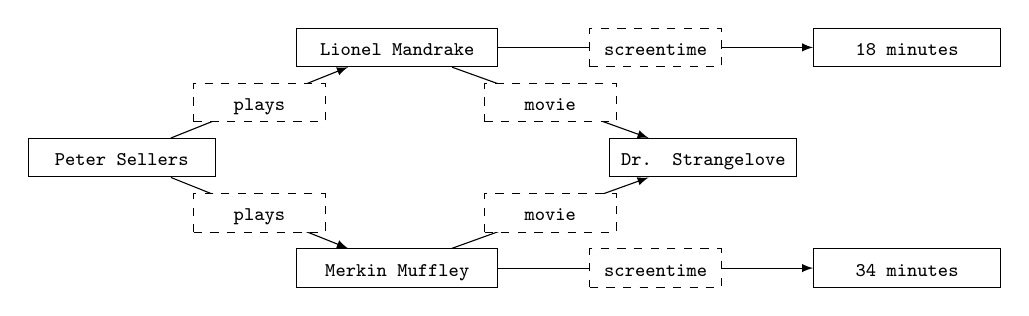
\begin{tikzpicture}
		
		%%%%% node n1 
		\node[rtt] (n1) {
			\al{60pt}{ 
				\uriq{Peter Sellers}}};
		
		%%%%% node n2 	
		\node[rtt,above=0.9cm of n1,xshift=3.5cm] (n2) {
			\al{65pt}{ 
				\uriq{Lionel Mandrake}}};	
		
		%%%%% edge e1
		\draw[arrout] (n1) to 
		node[ertt] (e1) 
		{\al{40pt}{
				\uri{plays}}}
		(n2);
		
		%%%%% node n3 	
		\node[rtt,below=0.9cm of n1,xshift=3.5cm] (n3) {
			\al{65pt}{ 
				\uriq{Merkin Muffley}}};	
		
		%%%%% edge e2
		\draw[arrout] (n1) to 
		node[ertt] (e2) 
		{\al{40pt}{
				\uri{plays}}}
		(n3);
		
		%%%%% node n4 
		\node[rtt,right=5cm of n1] (n4) {
			\al{60pt}{ 
				\uriq{Dr. Strangelove}}};    
		
		%%%%% edge e3
		\draw[arrout] (n2) to 
		node[ertt] (e3) 
		{\al{40pt}{
				\uri{movie}}}
		(n4);
		
		%%%%% edge e4
		\draw[arrout] (n3) to 
		node[ertt] (e4) 
		{\al{40pt}{
				\uri{movie}}}
		(n4);
		
		%%%%% node n5 
		\node[rtt,right=4cm of n2] (n5) {
			\al{60pt}{ 
				\uriq{18 minutes}}};
		
		%%%%% node n6 
		\node[rtt,right=4cm of n3] (n6) {
			\al{60pt}{ 
				\uriq{34 minutes}}};
		
		%%%%% edge e5
		\draw[arrout] (n2) to 
		node[ertt] (e5) 
		{\al{40pt}{
				\uri{screentime}}}
		(n5);
		
		%%%%% edge e6
		\draw[arrout] (n3) to 
		node[ertt] (e6) 
		{\al{40pt}{
				\uri{screentime}}}
		(n6); 
		\end{tikzpicture}
	\end{center}

\caption{An example of an edge-labelled graph. Reproduced from Angles et al \cite{ELGraphExample}.}
  \label{fig:ELGraph}
\end{figure}

\begin{figure}[ht]
\begin{center}

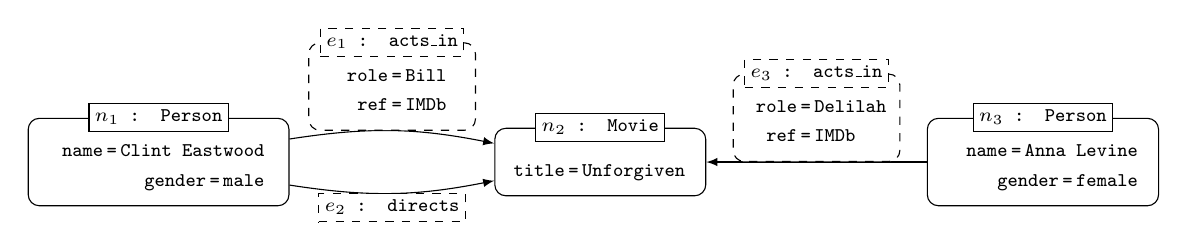
\begin{tikzpicture}
%%%%% node n1 
\node[rect] (n1) {
\alt{84pt}{
\urie{name} \uriq{Clint Eastwood}\\
\urie{gender} \uriq{male}}};

%%%%% label of n1
\node[rt] (ln1) at (n1.north) {\uri{$n_1$ : Person}};

%%%%% node n2
\node[rect, right=2.6cm of n1] (n2) {
\alt{66pt}{ 
\urie{title} & \uriq{Unforgiven}}};



%%%%% label of n2
\node[rt] (ln2) at (n2.north) {\uri{$n_2$ : Movie}};

%%%%% edge e1
\draw[arrout, bend left=10] (n1) to 
node[above, erect] (e1) {
\alt{50pt}{
\urie{role} \uriq{Bill}\\
\urie{ref} \uriq{IMDb}}}
(n2);



%%%%% label of e1
\node[ert] (le1) at (e1.north) {\uri{$e_1$ : acts\_in}};

%%%%% edge e2
\draw[arrout, bend right=10] (n1) to 
node[below, ert] (e2) {\uri{$e_2$ : directs}}
(n2);

%%%%% node n3
\node[rect, right=2.8cm of n2] (n3) {
\noindent
\alt{70pt}{
\urie{name} \uriq{Anna Levine}\\
\urie{gender} \uriq{female}}};

%%%%% label of n3
\node[rt] (ln3) at (n3.north) {\uri{$n_3$ : Person}};

%%%%% edge e3
\draw[arrin] (n2) to
node[above, erect] (e3) 
{
\alt{50pt}{
\urie{role} & \uriq{Delilah}\\
\urie{ref} & \uriq{IMDb}}}
(n3);

%%%%% label of e3
\node[ert] (le3) at (e3.north) {\uri{$e_3$ : acts\_in}};

\end{tikzpicture}

\end{center}
\caption{An example of a property graph. Reproduced from Angles et al \cite{PropertyGraphExample}}
  \label{fig:PropertyGraph}
\end{figure}



\subsection{Schema}
Current graph database systems often do not have rigid schema \cite{QueryLanguageSchema}. Instead, they use dynamic schema. This provides more flexibility in the shape of data that can be stored in the database; it also allows the types of nodes stored to evolve over time. The downside of this is that it requires additional typing checks at run-time. This also fails to fit into our definition of type-safety, since we have no guarantees about any objects extracted from the database. I have instead opted for a rigid schema which is built using Scala objects and is checked by the Scala compiler at compile-time.

\subsection{Mutability}
Current graph databases tend to be mutable. In order to express concepts that require immutability, such as time-dependent data, the user must impose extra constraints, such as adding time-stamps to the schema of  nodes and relations. A lack of immutability also complicates concurrent semantics and implementation of ACID (Atomic, Consistent, Independent, and Durable) transactions. I decided to introduce immutable data structures  to the database, which yields ACID properties effectively for free. This is explained in section \ref{immutability}.
\subsection{Query Languages}
Typically, database systems have their own query language, the most ubiquitous of which is Neo4j's language, Cypher \footnote{https://neo4j.com/docs/developer-manual/current/cypher/}. This provides ML-style pattern matching of queries against the stored graph, allowing the user to extract arbitrary fields from nodes. In most cases, theses are used by generating a query string and submitting it to the database engine. This is inherently not type-safe. The job of ensuring that absolutely every query a given program could generate is valid is intractable to undecidable for non-trivial programs. I decided to embed the query language in the host language. This allows the query language's type system to be checked by the host compiler, so we can get much stronger guarantees about program correctness.

\section{Immutability}\label{immutability}
In order to implement immutability, I needed a way of creating an immutable snapshot of the database at a given point in time. This is achieved using a system of views. A \codeName{View} is such an immutable snapshot. When we read from the database, we read from a particular given view. When we write to a particular view of the database, we copy the view, update it, and return the new view. Reads and writes now never interfere with each other. By utilising structure sharing, the impact of storing views can be mitigated.

\begin{figure}[ht]
\begin{center}
  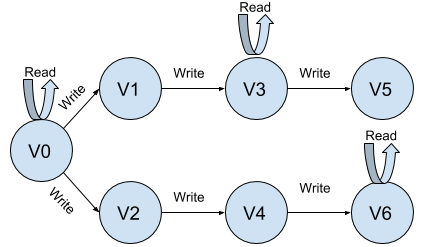
\includegraphics[width=\textwidth]{figs/readsWrites2.png}
  \caption{An example of reads and writes to an initial view. Separate reads and writes do not interfere with each other.}

\end{center}
  \label{fig:ReadsWrites}
\end{figure}

\section{Query Language}

In this next section, I shall define the query language that I constructed and introduce a set of semantics for evaluating queries.

\subsection{Domain Specific Language Syntax}
I spent some time iterating over a DSL syntax and how I wanted queries to look and be structured. My goals were to have a highly composable and expressive, yet small language. At first I experimented with a Neo4j-style language, with pattern matching syntax, an example of which is below. The query takes a number of fields to fill in, in this case a pair of actors, and finds all valid ways to fill them in subject to the graph constraints.
\renewcommand{\baselinestretch}{0.8}
\begin{framed}
\begin{verbatim}
 val coactor = RelationQuery {
    (x: Pattern[Actor], y: Pattern[Actor]) => {
       val m = ?[Movie]
        (x ~ ActsIn ~> m) && (y ~ ActsIn ~> m)
    }
}
\end{verbatim}
\note{Find two actors such they both act in the same movie}
\end{framed}
\renewcommand{\baselinestretch}{1.1}
This is fairly cluttered syntax and difficult to read. Furthermore, the Scala type inference system is fairly limited, meaning that users would frequently be required to insert type annotations in this syntax. It would also have been further complicated by adding the property graph features of Neo4j. Furthermore, we would not be able to easily and safely replicate Neo4j's ability to extract an arbitrary number of objects of different types from along a path defined by a query. Doing so would require use of structures such as heterogeneously typed lists.

As a result, I settled upon on an edge-labelled-relation-oriented approach which neatens the above query significantly.

\renewcommand{\baselinestretch}{0.8}
\begin{framed}
\begin{verbatim}
val coactor = ActsIn --><-- ActsIn
\end{verbatim}
\note{Find two actors such they both act in the same movie}
\end{framed}
\renewcommand{\baselinestretch}{1.1}

This is much more readable and concise. With this syntax, and the assumption that \codeName{ActsIn} relates \codeName{Actors} to \codeName{Movies}, Scala's typesystem can infer that \codeName{coactor} relates \codeName{Actors} to other \codeName{Actors}. There is also syntax for repetitions, intersections and unions. Examples of this syntax can be seen in appendix \ref{DSLExamples}.
\subsection{Semantic Definitions}\label{ADTDef}
To correctly implement the DSL, we need to mathematically model its operation. Hence, the above DSL queries should correspond to an intermediate representation. I have picked a set of expression constructors to do this. These fall into two kinds: \codeName{FindPair} and \codeName{FindSingle}, indicating whether they return pairs or individual values.

\paragraph{FindPair queries}
\begin{equation}
\label{PDefinition}
\begin{split}
P  &\rightarrow Rel(R) \mbox{ Find pairs related by the named relation R}\\
&\mid RevRel(R) \mbox{ Find pairs related by the named relation R in the reverse direction}\\
&\mid Chain(P, P) \mbox{   Find pairs related by the first subquery followed by the second}\\
&\mid And(P, P) \mbox{  Find pairs related by both of the sub-queries}\\
&\mid AndRight(P, S) \mbox{  Find pairs related by P where the right value is a result of s}\\
&\mid AndLeft(P, S) \mbox{  Find pairs related by P where the left value is a result of s}\\
&\mid Or(P, P) \mbox{  Find pairs related by either of the sub-queries}\\
&\mid Distinct(P) \mbox{  Find pairs related by P that are not symmetrical}\\
&\mid Id_A \mbox{ Identity relation}\\
&\mid Exactly(\mathit{n}, P) \mbox{  Find pairs related by n repetitions of P}\\
&\mid Upto(\mathit{n}, P) \mbox{  Find pairs related by upto n repetitions of P}\\
&\mid FixedPoint(P) \mbox{  Find the transitive closure of P}\\
\end{split}
\end{equation} 
where $n$ denotes a natural number. These queries look up a set of pairs of objects.\\

\paragraph{FindSingle queries}
\begin{equation}
\label{SDefinition}
\begin{split}
S & \rightarrow Find(F) \mbox{ Find values that match the findable F}\\
&\mid From(S, P) \mbox{ Find values that are reachable from results of S via P}\\
&\mid AndS(S, S) \mbox{ Find values that are results of both subqueries}\\
&\mid OrS(S, S) \mbox{ Find values that are results of either subquery}
\end{split}
\end{equation} 
Which look up sets of single objects.\\

\paragraph{Other Definitions}
In order to model the operation of queries correctly, we need to define the environment in which they operate.

\subparagraph{Object Types} are the ``real world'' types stored in the database. These correspond to the user's Scala classes.

\[ \tau \rightarrow A \mid B \mid C \mid .. \]

\subparagraph{Named relations} are the primitive relations between objects

\[R \rightarrow r_1 \mid r_2 \mid .. \]

\subparagraph{Findables} are names for defined partial functions

\[F_A \rightarrow f_1 \mid f_2 \mid ... \]

\[f \colon A \rightharpoonup \{True, False\} \]

For some given object type A. (i.e. a findable is an index into the database)

\subparagraph{A schema,}$\Sigma$, is made up of three partial functions:

\[\Sigma_{rel}\colon R \rightharpoonup \tau\times\tau \]
\[\Sigma_{findable}\colon F \rightharpoonup \tau \]
\[\Sigma_{table}\colon \tau \rightharpoonup \{True, False\} \]

Which give the types of relations and findables, and validiate the existence of a type. When it is obvious from the context, I shall simply use $\Sigma(x)$ to signify application of the appropriate function.
 
\subparagraph{A view,} $v \in V_\Sigma$, for a given schema $\Sigma$ represents an immutable state of a database.

It represents a pair of partial functions. Firstly the named-relation look up function.

\begin{equation}
v \in V_\Sigma \Rightarrow v_{rel}(r) \in \wp(A \times B)\mbox{ if $\Sigma(r)\downarrow (A, B)$}
\end{equation} 

That is, if a relation r is in the schema, then $v(r)$ is a set of pairs of objects with object type $\Sigma(r)$. Here, and from this point onwards I am using $\wp(s)$ to represent the power-set of a set, and $f(x) \downarrow y$ to mean $f$ is defined at $x$ and $f(x)=y$


The next function of a view is the type-look up function, it returns all objects in the view of a given object type:

\begin{equation}
v \in V_\Sigma \Rightarrow v_{table}(A) \in \wp(A)\indent \mbox{if $\Sigma(A)\downarrow True$}
\end{equation} 

That is, $v(A)$ is a set of objects of type $A$ stored in the view, and $A$ is a member of the schema $\Sigma$. Again I shall overload these two functions where it is clear from the context which is to be used.
 
\subsection{Typing}
In order to ensure the correctness of a given query, there is a type system to verify it. Typing rules take two forms. Firstly typing of pair queries:
\[ \Sigma \vdash P\colon (A, B)\]

Which means ``under the schema $\Sigma$, pair query $P$ returns a subset of $A \times B$''.  The second is for single queries:

\[ \Sigma \vdash S \colon A \]

Which means ``under the schema $\Sigma$ single query returns a subset of $A$''

The rules of the first kind are as follows

\begin{align}
&\displaystyle\mbox{(Rel)}\frac{\Sigma(r)\downarrow(A, B)}{\typeRule{Rel(r)}{(A, B)}} \\[3ex]
&\displaystyle\mbox{(Rev)}\frac{\Sigma(r)\downarrow(B, A)}{\typeRule{Rel(r)}{(A, B)}} \\[3ex]
&\displaystyle\mbox{(Id)}\frac{\Sigma(A)\downarrow True}{\typeRule{Id_A}{(A, A)}} \\[3ex]
&\displaystyle\mbox{(Chain)}\frac{\typeRule{P}{(A, B)} \indent \typeRule{Q}{(B, C)}}{\typeRule{Chain(P, Q)}{(A, C)}} \\[3ex]
&\displaystyle\mbox{(And)}\frac{\typeRule{P}{(A, B)} \indent \typeRule{Q}{(A, B)}}{\typeRule{And(P, Q)}{(A, B)}} \\[3ex]
&\displaystyle\mbox{(Or)}\frac{\typeRule{P}{(A, B)} \indent \typeRule{Q}{(A, B)}}{\typeRule{Or(P, Q)}{(A, B)}} \\[3ex]
&\displaystyle\mbox{(Distinct)}\frac{\typeRule{P}{(A, B)}}{\typeRule{Distinct(P)}{(A, B)}} \\[3ex]
&\displaystyle\mbox{(AndLeft)}\frac{\typeRule{P}{(A, B)} \indent \typeRule{S}{(A)}}{\typeRule{AndLeft(P,S)}{(A, B)}} \\[3ex]
&\displaystyle\mbox{(AndRight)}\frac{\typeRule{P}{(A, B)} \indent \typeRule{S}{B}}{\Sigma \vdash \typeRule{AndRight(P, S)}{(A, B)}} \\[3ex]
&\displaystyle\mbox{(Exactly)}\frac{\typeRule{P}{(A, A)}}{\typeRule{Exactly(n, P)}{(A, A)}} \\[3ex]
&\displaystyle\mbox{(Upto)}\frac{\typeRule{P}{(A, A)}}{\typeRule{Upto(n, P)}{(A, A)}} \\[3ex]
&\displaystyle\mbox{(FixedPoint)}\frac{\typeRule{P}{(A, A)}}{\typeRule{FixedPoint(P)}{(A, A)}} \\[3ex]
\end{align}


The rules for types of Single queries are similar:

\begin{align}
&\displaystyle\mbox{(Find)}\frac{\Sigma(f)\downarrow(A)}{\typeRule{Find(f)}{A}} \\[3ex]
&\displaystyle\mbox{(From)}\frac{\typeRule{P}{(A, B)} \indent \typeRule{S}{A}}{\typeRule{From(S, P)}{B}} \\[3ex]
&\displaystyle\mbox{(AndS)}\frac{  \typeRule{S}{A} \indent  \typeRule{S'}{A}}{\typeRule{AndS(S, S')}{A}} \\[3ex]
&\displaystyle\mbox{(OrS)}\frac{  \typeRule{S}{A} \indent  \typeRule{S'}{A}}{\typeRule{OrS(S, S')}{A}} \\[3ex]
\end{align}

\subsection{Semantics}
    To fully define the query language, we need to define the semantics. I have defined two collections of semantics: operational style and denotational style.
\paragraph{Operational Semantics}   

Now we shall define a set of rules for determining if a pair of objects is a valid result of a query. We're interested in forming a relation $a \triangleleft_A Q$ to mean``a is a valid result of query Q with type A''. This is dependent on the current view $v: View_{\Sigma}$. Hence we define $\opRule{(a, b)}{(A, B)}{P}$ for pair queries $P$ and $\opRule{a}{A}{S}$ for single queries $S$.

\begin{align}
&\displaystyle\mbox{(Rel)}\frac{(a,b) \in v(r)}{\opRule{(a, b)}{(A, B)}{Rel(r)}} \\[3ex]
&\displaystyle\mbox{(Rev)}\frac{(b,a) \in v(r)}{\opRule{(a, b)}{(A, B)}{RevRel(r)}} \\[3ex]
&\displaystyle\mbox{(Id)}\frac{a \in v(A)}{\opRule{(a, a)} {(A, A)} {Id_A}} \\[3ex]
&\displaystyle\mbox{(Distinct)}\frac{\opRule{(a,b)}{(A, B)}{P} \indent a \neq b}{\opRule{(a,b)}{(A, B)}{Distinct(P)}} \\[3ex]
&\displaystyle\mbox{(And)}\frac{\opRule{(a,b)}{(A, B)}{P} \indent \opRule{(a,b)}{(A, B)}{Q}}{\opRule{(a,b)}{(A, B)}{And(P, Q)}} \\[3ex]
&\displaystyle\mbox{(Or1)}\frac{\opRule{(a,b)}{(A, B)}{P}}{\opRule{(a,b)}{(A, B)}{Or(P, Q)}} \\[3ex]
&\displaystyle\mbox{(Or2)}\frac{\opRule{(a,b)}{(A, B)}{Q}}{\opRule{(a,b)}{(A, B)}{Or(P, Q)}} \\[3ex]
&\displaystyle\mbox{(Chain)}\frac{\opRule{(a,b)}{(A, B)}{P} \indent \opRule{(b,c)}{(B, C)}{Q}}{\opRule{(a,c)}{(A, C)}{Chain(P, Q)}} \\[3ex]
&\displaystyle\mbox{(AndLeft)}\frac{\opRule{(a,b)}{(A, B)}{P} \indent \opRule{a}{A}{S}}{\opRule{(a,b)}{(A, B)}{AndLeft(P, S)}} \\[3ex]
&\displaystyle\mbox{(AndRight)}\frac{\opRule{(a,b)}{(A, B)}{P} \indent \opRule{b}{B}{S}}{\opRule{(a,b)}{(A, B)}{AndRight(P, S)}} \\[3ex]
&\displaystyle\mbox{(Exactly_0)}\frac{\opRule{(a,b)}{(A, A)}{Id_A}}{\opRule{(a, b)}{(A, A)}{Exactly(0, P)}} \\[3ex]
&\displaystyle\mbox{(Exactly_{n+1})}\frac{\opRule{(a,b)}{(A, A)}{P} \indent \opRule{(b, c)}{(A, A)}{Exactly(n, P)}}{\opRule{(a, c)}{(A, A)}{Exactly(n + 1, P)}} \\[3ex]
&\displaystyle\mbox{(Upto_0)}\frac{\opRule{(a,b)}{(A, A)}{Id_A}}{\opRule{(a, b)}{(A, A)}{Upto(0, P)}} \\[3ex]
&\displaystyle\mbox{(Upto_n)}\frac{\opRule{(a, b)}{(A, A)}{Upto(n, P)}}{\opRule{(a, b)}{(A, A)}{Upto(n + 1, P)}} \\[3ex]
&\displaystyle\mbox{(Upto_{n+1})}\frac{\opRule{(a,b)}{(A, A)}{P} \indent \opRule{(b, c)}{(A, A)}{Upto(n, P)}}{\opRule{(a, c)}{(A, A)}{Upto(n + 1, P)}} \\[3ex]
&\displaystyle\mbox{(fix1)}\frac{\opRule{(a,b)}{(A, A)}{Id_A}}{\opRule{(a, b)}{(A, A)}{FixedPoint(P)}} \\[3ex]
&\displaystyle\mbox{(fix2)}\frac{\opRule{(a,b)}{(A, A)}{P} \indent \opRule{(b, c)}{(A, A)}{FixedPoint(P)}}{\opRule{(a, b)}{(A, A)}{FixedPoint(P)}} \\[3ex]
\end{align}

And the FindSingle rules

\begin{align}
&\displaystyle\mbox{(Find)}\frac{a \in v(A) \indent f(a)\downarrow True}{\opRule{a}{A}{Find(f)}} \\[3ex]
&\displaystyle\mbox{(From)}\frac{\opRule{a}{A}{S} \indent \opRule{(a,b)}{)(A, B)}{P}}{\opRule{b}{A}{From(S, P)}} \\[3ex]
&\displaystyle\mbox{(AndS)}\frac{\opRule{a}{A}{S} \indent \opRule{a}{A}{S'}}{\opRule{a}{A}{And(S, S')}} \\[3ex]
&\displaystyle\mbox{(OrS1)}\frac{\opRule{a}{A}{S}}{\opRule{a}{A}{Or(S, S')}} \\[3ex]
&\displaystyle\mbox{(OrS1)}\frac{\opRule{a}{A}{S'}}{\opRule{a}{A}{Or(S, S')}} \\[3ex]
\end{align}
\paragraph{Denotational Semantics}
The operational semantics clearly demonstrate membership of a query, but do not give a means to efficiently generate the results of query. To this end, we introduce denotations $\llbracket P \rrbracket$ and $\llbracket S \rrbracket$ such that \[\Sigma \vdash P \colon (A, B) \Rightarrow\llbracket P \rrbracket \colon View_{\Sigma} \rightarrow \wp(A \times B)\]

and \[\Sigma \vdash S \colon A \Rightarrow\llbracket S \rrbracket \colon View_{\Sigma} \rightarrow \wp(A)\] Such denotations should be compositional and syntax directed, whilst still corresponding to the operational semantics.

\begin{align}
& \deno{Rel(r)} = v(r) \\[3ex]
& \deno{RevRel(r)} = swap(v(r)) \\[3ex]
& \deno{Id_A} = dup(v(A)) \\[3ex]
& \deno{Chain(P, Q)} = join(\deno{P}, \deno{Q}) \\[3ex]
& \deno{And(P, Q)} = \deno{P} \cap \deno{Q} \\[3ex]
& \deno{Or(P, Q)} = \deno{P} \cup \deno{Q} \\[3ex]
& \deno{AndLeft(P, S)} = filterLeft(\deno{P}, \deno{S}) \\[3ex]
& \deno{AndRight(P, S)} = filterRight(\deno{P}, \deno{S}) \\[3ex]
& \deno{Distinct(P)} = distinct(\deno{P}) \\[3ex]
& \deno{Exactly(n, P)} = (\lambda pairs. join(\deno{P}, pairs))^n \deno{Id_A} \\[3ex]
& \deno{Upto(n, P)} = (\lambda pairs. join(\deno{P}, pairs) \cup pairs)^n \deno{Id_A} \\[3ex]
& \deno{FixedPoint(P)} = fix (\lambda pairs. join(\deno{P}, pairs) \cup pairs)  \mbox{ in the domain $\clos$}\\[3ex]
\end{align}

And similarly with single queries

\begin{align}
&\deno{Find(f)} = \setComp{a \in v(A)}{f(a)\downarrow True} \mbox{ for $\Sigma(f) = A$} \\[3ex]
&\deno{From(S, P)} =  \setComp{b}{(a, b) \in \deno{P} \&\wedge a \in \deno{S}}   \\[3ex]
&\deno{AndS(S, S')} = \deno{S} \cap \deno{S'} \\[3ex]
&\deno{OrS(S, S')} = \deno{S} \cup \deno{S'} \\[3ex]
\end{align}
with the following definitions:
\[ swap(s) = \setComp{(b,a)}{(a, b) \in s}\]
\[ dup(s) = \setComp{(a,a)}{a \in s}\]
\[ join(p, q) = \setComp{(a, c)}{ \exists b. (a, b) \in p \wedge (b, c) \in q}\]
\[ distinct(s) = \setComp{(a, b) \in s} { a \neq b} \]
\[ filterLeft(p, s) = \setComp{(a, b) \in p}{a \in s}\]
\[ filterRight(p, s) = \setComp{(a, b) \in p}{b \in s}\]
    
   I have also proved in appendix \ref{DenoOper} the correspondence of these two formulations of semantics.
\subsection{Commands}
In addition to the query construction language, there are five commands which make use of the queries.

\[\label{CommandSemantics}
\begin{split}
findPairs(P, v) &= \deno{P}\\
find(S, v) &=  \deno{S}\\
shortestPath(a, a', P, v) &= \mbox{An \codeName{Option} of Shortest path, if it exists, from $a$ to $a'$}\\
& \indent \mbox{in the graph defined by $\deno{P}$}\\
allShortestPaths(a, P, v) &= \mbox{The set of the shortest path to each element reachable}\\
 & \indent \mbox{from $a$ in the graph defined by $\deno{P}$}\\
\end{split}\]

The definition of the write command is slightly more complicated. It needs to return an updated view with its look up functions now returning the inserted objects. Write takes a collection, $rs$, of correctly typed named relations instances.


\[rs = \setComp{(a_i, r_i, b_i) \in (A \times R \times B)}{0 < i \leqslant n} \mbox{for some $n$ being the size of the set.}\]
and updates the view as so: 
\begin{equation}
\begin{split}
write(rs, v) = &v\left[A \mapsto v_{table}(A) \cup \setComp{a_i}{0 < i \leqslant n}\right]\\
& \left[B \mapsto v_{table}(B) \cup \setComp{b_i}{0 < i \leqslant n}\right]\\
& \left[r \mapsto v_{rel}(R) \cup \setComp{(a_i, b_i)}{0 < i \leqslant n}\right] 
\end{split}
\end{equation}

\subsection{Summary}
To summarise, this past section defines a query DSL, a type system for checking validity of queries, and a set of semantics for executing queries. Furthermore, I have then defined a set of commands which allow queries to execute and views to be generated.


\section{Starting Point}
In addition to Scala, I have made use of several libraries and tools, some of which were not forseen in my project proposal. Some were used for the actual construction of the project, whereas others were used for auxiliary tasks such as testing and debugging or  generating datasets. All of these tools have licenses allowing free usage (The exact license for each is given in the footnotes.) and no modifications to these libraries were performed.\\

\begin{tabular}{p{4cm}p{11cm}}
\textbf{SBT}\footnote{//www.Scala-sbt.org/} & Scala Build Tool (SBT) is a package manager and build tool for Scala which allows access to Java libraries. \footnote{https://github.com/sbt/sbt/blob/1.x/LICENSE}\\
\\
\textbf{PostgreSQL}\footnote{//www.postgresql.org/} & An open-source, multi-platform SQL implementation.\footnote{https://opensource.org/licenses/postgresql}\\\\

\textbf{LMDB}\footnote{//symas.com/lmdb/}&An open source, highly optimised key-value datastore. \footnote{http://www.openldap.org/software/release/license.html}\\\\

\textbf{Scalaz}\footnote{https://github.com/Scalaz/Scalaz} & A library for Scala providing typeclasses and syntax to aid advanced functional programming.\footnote{https://github.com/scalaz/scalaz/blob/series/7.3.x/LICENSE.txt} \\\\

\textbf{JDBC}\footnote{http://www.oracle.com/technetwork/java/javase/jdbc/index.html} & Java's standard library support for SQL connections. Used to interact with a postgres database. I had originally planned to use the higher level wrapper scalikeJDBC,\footnote{http://scalikejdbc.org/} however, this did not allow such fine control over queries as I would have liked. \footnote{https://jdbc.postgresql.org/about/license.html}\\\\

\textbf{LMDBJava}\footnote{//github.com/lmdbjava/lmdbjava} & A JNI library allowing access to the LMDB datastore. Previously, I experimented with another library, LMDBJni. However, upon discovery of a bug in the JNI code, I switched to LMDBJava.\footnote{https://github.com/lmdbjava/lmdbjava/blob/master/LICENSE.txt}\\\\

\textbf{Junit}\footnote{https://junit.org/junit5/} & A unit testing library for JVM languages.\footnote{https://junit.org/junit4/license.html}\\\\

\textbf{SLF4J}\footnote{https://www.slf4j.org/} & A logging library for JVM languages. \footnote{https://www.slf4j.org/license.html} \\\\

\textbf{Spray-JSON}\footnote{https://github.com/spray/spray-json}& A JSON library for Scala, used to generate benchmarking datasets. \footnote{https://github.com/spray/spray-json/blob/master/LICENSE} \\\\

\textbf{Python}\footnote{https://www.python.org/} & A scripting language used to generate test datasets. \footnote{https://docs.python.org/3/license.html}
\\\\

\end{tabular}


\section{Software Engineering}

\begin{figure}[ht]
\centering
  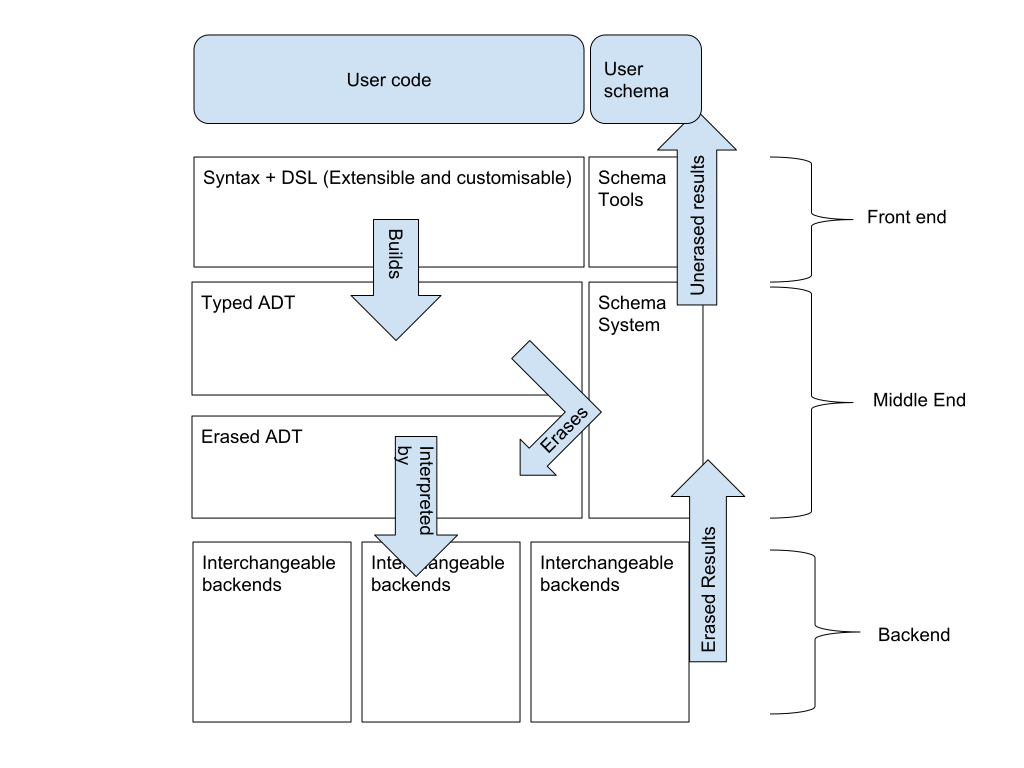
\includegraphics[width=\textwidth]{figs/Architecture.png}
  \caption{A map of the architecture of the system}
  \label{fig:Architecture}
\end{figure}
The system was designed to be as modular and re-implementable as possible. To this end, it consists of several interchangeable components; a map of this is provided in figure \ref{fig:Architecture}. The front-end mostly consists of interfaces and syntax for building queries and the schema for the database. The front-end's DSL translates into the underlying typed ADT. This then has its compile-time type information erased to become an un-typed query ADT, which is easier and cleaner to interpret. Finally, there are three interfaces that a back-end system must implement: DBBackend, DBInstance and DBExecutor. These specify a root back-end object that opens an instance which represents a database connection. Each DBInstance has an executor that allows us to execute commands. The results of these commands are then un-erased to return them as the correct type.

I progressed through the project using an iterated waterfall method. Each time it came to add a new module, such as a back-end, I planned the overall execution method and storage structure, then wrote the interfaces for submodules. Next, I filled in the components and tested the new back-end against a growing set of unit and regression tests.

\section{Scala Techniques}
I have made use of several advanced programming techniques which are specific to the Scala language.

\subsection{Type-Enrichment}
The type-enrichment feature of the Scala language allows retroactive addition of methods to previously defined types. type-enrichment is performed by creating an implicit class, taking a single underlying value of some given type. The methods defined in the implicit class can now be called as if they were methods of the underlying class, provided the implicit class is in scope.

\renewcommand{\baselinestretch}{0.8}
\begin{framed}
\begin{framed}
\begin{verbatim}
object Outer {
    implicit class EnrichInt(i: Int){
        def neg: Int = -i
        def  succ: Int = i + 1
        def mod(n: Int) = i - (i / n)*n
    }
}
\end{verbatim}
\end{framed}
\renewcommand{\baselinestretch}{1.1}
When Outer is imported, we can now do

\renewcommand{\baselinestretch}{0.8}
\begin{framed}
\begin{verbatim}
5.neg == -5
6.succ == 7
10 mod 4 == 2
\end{verbatim}
\end{framed}
\end{framed}
\renewcommand{\baselinestretch}{1.1}






This allows us to add syntax to types where a small number of core methods have been defined.

\subsection{Implicit Parameters}
Another advanced feature of Scala that  I have used is that of implicit  parameters to functions and class constructors. Values such as vals, functions, and classes can be declared with an implicit tag. Functions and classes can declare additional parameters as implicit. When these functions are called, the implicit parameter can be omitted if and only if there is an unambiguous implicit value of the correct type in scope.

\renewcommand{\baselinestretch}{0.8}
\begin{framed}
\begin{framed}
\begin{verbatim}
object foo {
    implicit val i = 5
}

object bar {
    def plusImpl(j: Int)(implicit k: Int): Int = j + k
}
\end{verbatim}
\end{framed}

\begin{framed}
\begin{verbatim}
import foo._

bar.plusImpl(4) == 9
\end{verbatim}
\end{framed}
\end{framed}
\renewcommand{\baselinestretch}{1.1}

This is typically used for purposes such as passing around values that are defined once and used many times in a program, such as an execution context, or a logging framework instance.

Functions can also be implicit and take implicit values
\begin{framed}
\begin{verbatim}
implicit def f(implicit a: A): B = ...
\end{verbatim}
When an implicit value of type A is available, then an implicit value of type B is also available.
\end{framed}

This can be made more interesting when we include parameterised generic types. This allows us to get the compiler to do work in the manner of an automated theorem prover (by the Curry-Howard correspondence) at compile-time.

\renewcommand{\baselinestretch}{0.8}
\begin{framed}
	\begin{framed}
		\begin{verbatim}
		
object Defs {
    implicit val s: String = "foo"
    implicit val i: Int = 2
    Implicit def toList[A](implicit a: A): List[A] = List(a, a, a)

    def getImplicit[A](implicit a: A): A = a
}
		\end{verbatim}
	\end{framed}
	\begin{framed}
		\begin{verbatim}
		import Defs._

getImplicit[List[Int]] == List(2, 2, 2)
getImplicit[List[List[String]] == 
        List(List(“foo", “foo", "foo"),
        List("foo", "foo", "foo"), 
        List("foo", "foo", "foo"))
		\end{verbatim}
	\end{framed}
\end{framed}
\renewcommand{\baselinestretch}{1.1}


\subsection{Typeclass Pattern}
A further combination of these two patterns is the typeclass pattern. We define a typeclass for a type by defining as methods on a trait the operations we want on the type. We can then define implicit objects which work as type class instances for the types we want. We can also use implicit functions to generate typeclass instances in a manner similar to a proof tree. We can then use the type-enrichment feature to add methods to values of a type that is a member of the typeclass.

\renewcommand{\baselinestretch}{0.8}
\begin{framed}
	\begin{framed}
		\begin{verbatim}
trait Monoid[A] {
     def id: A
     def op(a1: A, a2: A): A
}
		\end{verbatim}
	\end{framed}
	
	Definition of a monoid typeclass instance using F-type polymorphism
	
	\begin{framed}
		\begin{verbatim}
object Instances {
  implicit object IntMonoid extends Monoid[Int] {
    override val id: Int = 0
    override def op(a1: Int, a2: Int): Int = a1 + a2
  }

  implicit def ListMonoid[A] = new Monoid[List[A]] {
    override val id: List[A] = List()
    override def op(a1: List[A], a2:  List[A]):  List[A] =
      a1 ++ a2
    }
 

  implicit def PairMonoid[A, B](
    implicit MA: Monoid[A], MB: Monoid[B]
  ) = new Monoid[(A, B)]{
    override val id: (A, B) = (MA.id, MB.id)
    override def op(p: (A, B), q: (A, B)) =
      (MA.op(p._1, q._1), MB.op(p._2, q._2))
  }
}
	\end{verbatim}
	\end{framed}
	
	Definition of several monoid instances, including a pair monoid that combines monoids.
	
	\begin{framed}
		\begin{verbatim}
		
object Syntax {
  implicit class MonoidOps[A](a: A)(implicit ma: Monoid[A]) {
     def *(n: Int): A = if (n == 0) ma.id else ma.op(a, *(n-1))
  }
}
		\end{verbatim}
	\end{framed}
Definition of a multiplication operation on instances of a monoid.
	\begin{framed}
		\begin{verbatim}
			 (5, List("f")) * 3 == (15, List("f", "f", "f"))
		\end{verbatim}
	\end{framed}
Usage of the multiplication operation on a tuple.
\end{framed}
\renewcommand{\baselinestretch}{0.8}

It is clear that these patterns allow for very expressive structures and abstractions to be built in Scala. I use these frequently within the project to neaten code and to achieve type-safety.



\chapter{Implementation}

In this section, I shall first focus on common techniques when building the database, then explain construction of the front- and middle-ends. After this, I shall look at common structures shared by the various back-end implementations and finally, I shall conclude with an examination of each of the back-end implementations that I have written. 
\section{Note on Purity and Concurrency}
All of the back-ends aim to preserve the global immutability of the database. The immutable semantics of the database also mean that queries generally do not interfere with each other. This means that we can avoid keeping locks or creating large transactions. Hence, the back-ends do not require much work to maintain correct concurrency.
\section{Functional Programming Techniques}
	\subsection{Monadic Compilation}\label{MonadicCompilation}
	At several points in building a back-end, it becomes necessary to transform one algebraic type to another. This is typically performed by walking over a tree, whilst keeping some mutable state representing parts of the tree that are relevant. One example is converting an intermediate representation to SQL output code. Here, we may want to extract common sub-expressions into a dictionary, or pick out all the database tables that need to be accessed by the query. This can be encoded by folding a State Monad instance over the tree.

The state monad is an abstraction over functions that chain an immutable state through successive computations.

\renewcommand{\baselinestretch}{0.8}
\begin{framed}
\begin{verbatim}
class State[S, A](r: S => (S, A)) {
      def runState(s: S): (S, A) = r(s)
}


object Example {
  Implicit def StateMonadInstance[S] = new Monad[State[S, _]] {
     def point[A](a: A) = new State(s => (s, a))
     def bind[A, B](sa: State[S, A], f: A => State[S, B]) = new State(
        s => {
          val (s', a) = sa.runState(s)
          f(a).runState(s')
        }           
      )
    }
  }
\end{verbatim}
\end{framed}
\renewcommand{\baselinestretch}{1.1}

To define a monadic compiler, we define a recursive function which chains state monad objects together.

\renewcommand{\baselinestretch}{0.8}
\begin{framed}
\begin{verbatim}
def compile(adt: ADT): State[S, Res] = adt match {
   case basis => ...
   case Pattern(a, b) => for {
      ca <- compile(a)
      cb <- compile(b)
   } yield foo(ca, cb) 
}
\end{verbatim}
\end{framed}


	\subsection{Constrained Future Monad}
	Part of the goal of type-safety is the recovery of error cases. Typically, this would be handled in a JVM program through the use of exceptions. However the presence of unchecked exceptions on the Java platform makes it difficult to ensure that all error cases are accounted for. A more functional approach is the use of the exception monad \cite{ExceptionMonad}. In Scala, this manifests as the built in Try monad and Scalaz's \codeName{\either} (\codeName{Either}) monad. \codeName{Try[A]} has two case classes: \codeName{Failure(e: Throwable)} and \codeName{Success(a: A)}, while \codeName{E \either A} has the case classes \codeName{\eitherL(e: E)} and \codeName{\eitherR(a: A)} (\codeName{Left} and \codeName{Right}). Since \codeName{Try}'s failure case is the unsealed \codeName{Throwable} trait, we do not really have a way to ensure we have handled all error cases at compile-time, whereas \codeName{Either} has a parametrised error type, which can be a sealed type hierarchy, which is then checked by the Scala compiler at run-time. For example, consider the simple interpreter below. All error cases are proved to be handled by the type-system.

\renewcommand{\baselinestretch}{0.8}
\begin{framed}
	\begin{framed}
		\begin{verbatim}
			sealed trait Error
			case object DivByZero extends Error
			case object Underflow extends Error

			sealed trait NoError
		\end{verbatim}
	\end{framed}
	
	A simple pair of error hierarchies. One signifying errors, and NoError indicating a lack of error. Note that $NoError$ cannot be instantiated or sub-classed.


	\begin{framed}
		\begin{verbatim}
def eval(e: Expr): Error \/ Int = 
  e match {
    case Div(a, b) => for {
        aRes <- eval(a)
        bRes <- eval(b)
        r <- if (bRes == 0) DivByZero.left else (aRes/bRes).right
      } yield r

    case Sub(a, b) => for {
        aRes <- eval(a)
        bRes <- eval(b)
        r <- if(bRes > aRes) Underflow.left else (aRes-bRes).right
    } yield r
}
		\end{verbatim}
	\end{framed}
\renewcommand{\baselinestretch}{1.1}
	
	A simple interpreter for a simple algebraic datatype for expressions that returns an error or a result
	
\renewcommand{\baselinestretch}{0.8}
	\begin{framed}
		\begin{verbatim}
def evalAndPrint(e: Expr): NoError \/ String = 
  eval(e) match {
    case \/-(i) =>i.toString.right
    case -\/(e) => e match {
        case DivByZero => “division by zero”.right
        case UnderFlow => “underflow”.right
    }
  }
		\end{verbatim}
	\end{framed}
\renewcommand{\baselinestretch}{1.1}

	A simple result printer that correctly handles all error cases and reduces its error parameter to the un-instantiable $NoError$ type
		
\end{framed}


Typically, we deal with cases which might take a significant amount of time to return. So rather than using a simple \codeName{Either} monad, we lift it into an asynchrony monad. There are several options to choose from for an asynchrony monad. I chose the built in \codeName{Future} over more exotic alternatives, such as the Scalaz \codeName{Task}, since it is relatively widely used, and I have some familiarity with it from past projects. \codeName{Futures} also capture thrown unchecked exceptions, which makes handling them a little easier. Hence we are interested in passing around \codeName{Future[E \either A]} around, for a sealed type hierarchy \codeName{E}. There is also the issue of the Java libraries used (for SQL and LMDB access) throwing exceptions, and unexpected exceptions turning up in code. Fortunately, the  Future container catches these, acting like an asynchronous \codeName{Try[E \either A]}. This causes issues as we do not have the sealed trait property of errors as we have above. To solve this, I introduced the \codeName{ConstrainedFuture[E, A]} monad, which has the requirement that the error case type parameter \codeName{E} implements the \codeName{HasRecovery} typeclass for converting any \codeName{Throwable} to an \codeName{E}.

\renewcommand{\baselinestretch}{0.8}
\begin{framed}
	\begin{verbatim}
trait HasRecovery[E] {
 def recover(t: Throwable): E
}
	\end{verbatim}
\end{framed}
\renewcommand{\baselinestretch}{1.1}

The underlying future is kept private, and can only be accessed via the run method, which calls the recover method on any errors (tail recursively, so any exceptions thrown during execution are also handled). By this construction, we ensure all non-fatal error cases are contained in a type-safe way.

	\subsection{Operation Monad}
	As stated in section \ref{immutability}, typical database operations take a view as a parameter, inspect the view, return a value and may also insert a new view. This requires interplay between the \codeName{ConstrainedFuture} (to handle failure and asynchrony) and \codeName{State} (to chain together updates to the view representing current state) monads. Hence we use the \codeName{Operation[E, A]} monad, which wraps a function \codeName{$(ViewId \Rightarrow ConstrainedFuture[E, (ViewId, A)])$} in a similar way to how \codeName{State} monad chains together functions \codeName{$S \Rightarrow (S, A)$}. Each of the commands on a database yields an operation.

	
	\subsection{Local and Global State}
Although it would be preferable to only use purely functional folds, maps, and immutable data structures everywhere within the project, for certain, high frequency, performance critical tasks, using purely immutable structures slows us down. Recursive functions (though my functional style does not make heavy use of them anyway) tend to use more stack space than the JVM has available in many situations. Hence for tasks such as retrieving values for result sets,  pathfinding across large relations, and building indices, I have opted to make use of mutable data structures locally, using builders \footnote{https://docs.scala-lang.org/overviews/core/architecture-of-scala-collections.html\#builders} for collections such as sets. This leads to a dramatic increase in speed, especially for when large numbers of elements are added sequentially to collections that are not lists. In these cases, the mutable state never leaks out of the functions that make use of the mutability.	
	
\section{Schema Implementation}
	One of the goals of the project was to allow close to arbitrary user objects (assuming that they are finite) to be inserted and retrieved from the database. This was achieved using the typeclass pattern.
	\subsection{Schema Hierarchy}
	In order to work with the database, a class needs to have an instance of the \codeName{SchemaObject} typeclass.

\renewcommand{\baselinestretch}{0.8}
	\begin{framed}
		\begin{verbatim}
sealed trait SchemaObject[A] {
// components for constructing DB
 def schemaComponents: Vector[SchemaComponent]  tables
 def any: Pattern[A] // Findable that matches any A
 def findable(a: A): DBTuple[A] // convert an object to a findable
 def name: TableName // name of the table
 def fromRow(row: DBObject): ExtractError \/ A // unmarshall an A
}
		\end{verbatim}
	\end{framed}
\renewcommand{\baselinestretch}{1.1}
	
	\codeName{SchemaObject} is sealed, so can only be implemented by implementing one of its subclasses. Currently, for the sake of simplicity, there are five: \codeName{SchemaObject0} .. \codeName{SchemaObject4}, with the number indicating the number of underlying database fields required. These simplify the construction of a type-class instance to marshalling values of the object type to tuples of  \codeName{Storable}, primitive types. Examples can be seen in appendix \ref{SchemaObjectDemo}
	
	\subsection{DBObjects}
	
	To store objects in the database under various back-ends, we need to have a type erased (at compile-time, but not run-time) version of the objects. Once we have a primitive representation of an object from the \codeName{SchemaObject}, we can fully unerase it by converting it to a \codeName{DBObject}. A \codeName{DBObject} is simply a collection of type tagged fields (\codeName{DBCell}). These can now be easily inserted or retrieved from a database.
	
\renewcommand{\baselinestretch}{0.8}
\begin{framed}
	\begin{verbatim}
type DBObject = Vector[DBCell]

type DBCell -> DBInt of Int 
			| DBString of String
			| DBBool of Boolean
			| DBDouble of Double
	\end{verbatim}
	
	\note{Pseudo-ml definitions of \codeName{DBObject} and its components}
\end{framed}
\renewcommand{\baselinestretch}{0.8}
	
	\subsection{Unerasure}
	In order to correctly retrieve values from the database, we need to be able to undo the erasure process. This can be performed using the unmarshalling methods derived from the \codeName{SchemaObject}  for an object type.
	\subsection{Relations}
	    In order for type checking to work, relations need to have type parameters for the object types they link. Hence, to define relations in the schema, the user needs to define objects that extend the relation interface.
	    
\renewcommand{\baselinestretch}{0.8}
\begin{framed}
\begin{verbatim}
abstract class Relation[A, B](
    implicit val sa: SchemaObject[A], val sb: SchemaObject[B]
) extends FindPairAble[A, B]
\end{verbatim}
\end{framed}
\renewcommand{\baselinestretch}{1.1}



	
	\subsection{SchemaDescription}
	
In order to build the database structures the back-ends need a definitive collection of schema to include. This is performed using a \codeName{SchemaDescription} object, which simply holds a collection of \codeName{SchemaObjects} and \codeName{Relations} which need to be used by the database.	
	
	\subsection{Findables}
	For the sake of simplicity, I have only implemented findables which test if fields of objects match particular values. This allows us to look for specific objects or match particular fields. This also makes indexing easier to implement.
	
\section{Query ADT}
The intermediate representation terms described in  section \ref{ADTDef} are implemented in Scala by a pair of ADT hierachies: a typed and type-erased equivalent for each. The typed ADTs are parameterised by the object types which they look up. Using this parameterisation, I have encoded in type of the ADTs the inductive type rules in the semantics such that the Scala compiler checks the type of any generated query and does type inference for us. The definitions of these Scala classes can be found in appendix \ref{ScalaADT} The only rules that cannot be checked at compile-time are whether the schema description contains the relation in instances of the (\codeName{Rel}) rule, the type \codeName{A} for the (\codeName{$Id_A$}) rule, and the (\codeName{Find}) rule, as we cannot predict the contents of the SchemaDescription at compile-time without dependent types.  The typed ADTs are erased, with respect to a schema,  into their unsafe equivalents in order to be executed. If an AST node makes reference to a non-existent table or relation, a run-time error is created in the \codeName{Either} return type. The constructors of the type-erased ADT nodes are private to the enclosing package, meaning that they can only be created by erasing a typed ADT.
	
\section{Commands}
As specified in the previous chapter, each back-end needs to implement five commands: 
\begin{itemize}
\item \codeName{find(S): Operation[E, Set[A]]}
\item \codeName{findPairs(P): Operation[E, Set[(A, B)]]}
\item \codeName{ShortestPath(start, end, P): Operation[E, Option[Path[A]]}
\item \codeName{allShortestPaths(start, P): Operation[E, Set[Path[A]]}
\item \codeName{insert(relations): Operation[E, Unit]}.
\end{itemize}
Each command should return an \codeName{Operation} of the correct type.
\section{DSL}
The DSL mostly consists of syntactic sugar to make queries easier to read. It is implemented using the type-enrichment pattern. Both \codeName{Relation} and \codeName{FindPair} implement the trait (interface) \codeName{FindSingleAble}, so we can use type-enrichment to write new DSL opertors. The main thing to note in the DSL is the use of arrows to chain relations together. Examples of the DSL can be seen in appendix \ref{DSLExamples}

\section{Common Generic Algorithms}
During construction of the database, several common patterns of problems emerged with slight differences. Hence, I have written relatively optimised generic versions of these algorithms such that different back-ends can make use of them regardless of the underlying types. These algorithms are found in \codeName{core.utils.algorithms}


	\subsection{Simple Traversal}\label{SimpleFixedPoint}
	The first set of generic algorithms to look at are the \codeName{SimpleFixedPointTraversal} algorithms. These compute the repetitions of a function for execution of the \codeName{FixedPoint}, \codeName{Upto}, and \codeName{Exactly} expressions of the ADT. They are labelled as "Simple" because they do the search from a single root. They carry out search mutably, and convert their output to an immutable set upon returning.
	
		\paragraph{Exactly}
The simplest algorithm is for computing \codeName{Exactly} query nodes. Here, we simply expand a fringe set of values outwards, by applying the search step to every value in the fringe to get the new fringe. We also memoise the search step function in the case of repetitions. After the required number of repetitions, the remaining fringe is returned. An illustration can be found in \ref{fig:ExactlySingle}.

\begin{figure}[ht]
\centering
  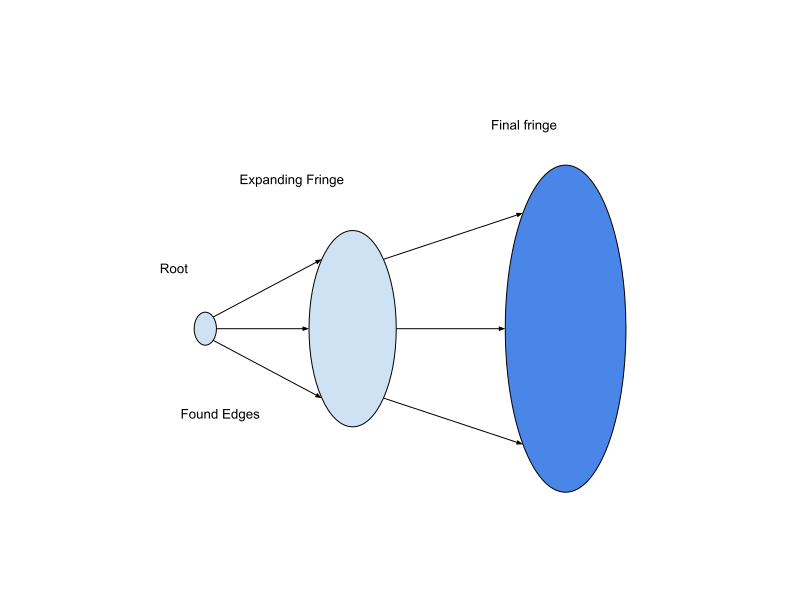
\includegraphics[width=\textwidth]{figs/Exactly.png}
  \caption{Execution of a simple \codeName{Exactly} query}
  \label{fig:ExactlySingle}
\end{figure}
    		\paragraph{Upto}
The next algorithm is for computing \codeName{Upto}. This is computed in a similar way by flat-mapping the functions over the fringe repeatedly to calculate an expanding fringe. The major differences here are that we keep an accumulator of all the found values. When a new fringe is calculated, we subtract the accumulator set from it to reduce the number of nodes that need to be searched to those that have not yet been searched, and then union the remaining fringe with the accumulator to get the new accumulator. After the required number of repetitions, the accumulator is returned. An illustration can be found in \ref{fig:UptoSingle}.

\begin{figure}[ht]
\centering
  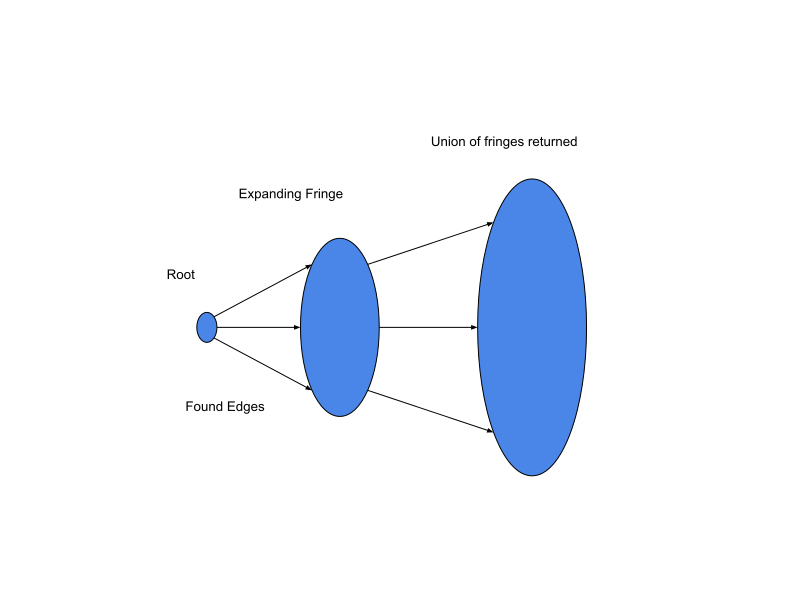
\includegraphics[width=\textwidth]{figs/Upto.png}
  \caption{Execution of a simple \codeName{Upto} query}
  \label{fig:UptoSingle}
\end{figure}
	
		\paragraph{FixedPoint}
The  final algorithm is to calculate \codeName{FixedPoint}. This works slightly differently. As before, we keep an accumulator of reached nodes, but unlike before, the generation number of each node is not important, only that a node is reachable is important. Hence, the fringe is a queue rather than a set, and we iterate until the fringe is empty. In each iteration, we pop off the top value of the fringe queue, compute all immediately reachable nodes. The difference of this reachable set is taken with the accumulator to find the newly reached nodes. These are now added to the fringe queue and the accumulator. When the fringe is empty, we return the accumulator.
	
	\subsection{Full traversal}
		The next set of algorithms build on the \codeName{SimpleFixedPoint} algorithms to return not just those nodes reachable from a single root, but the set of all reachable pairs with the left hand pair derived from a root set (using the left-hand optimisation explained is section \ref{leftOpt}). As such, the algorithms need to do some more work to reconstruct which nodes are reachable from each root, while still eliminating redundancies.
		\paragraph{Exactly}
The first such algorithm is for computing \codeName{Exactly}. This is similar to the original version, except we now store a fringe for each root in a map of \codeName{Root => Set[Node]}. We also memoise the search function in a Map to avoid computing it redundantly. In each iteration, we simply expand the fringe for each root as before by mapping the fringe expansion loop body over the values of the fringe map. An illustration can be found in \ref{fig:ExactlyPairs}.

\begin{figure}[ht]
\centering
  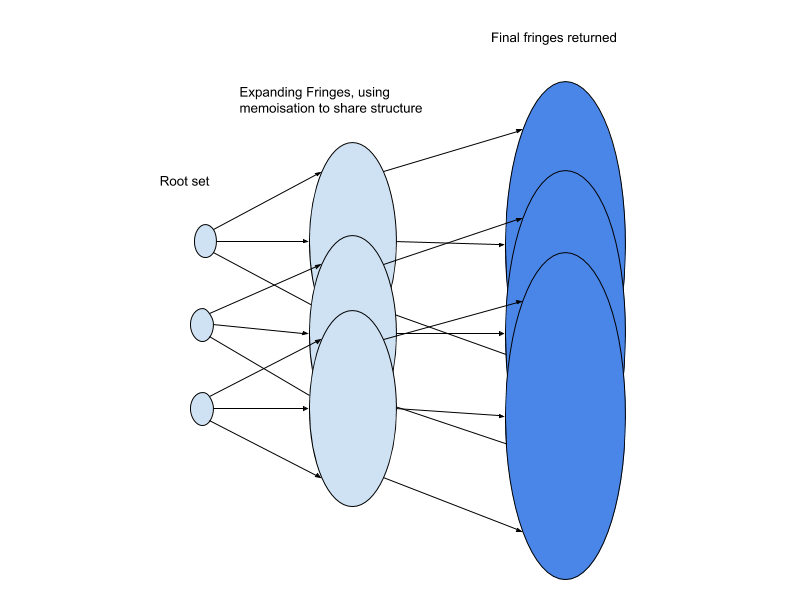
\includegraphics[width=\textwidth]{figs/ExactlyPairs.png}
  \caption{Execution of an \codeName{Exactly} query from multiple roots}
  \label{fig:ExactlyPairs}
\end{figure}
		
		\paragraph{Upto}
The next algorithm is to compute \codeName{Upto}. This is again accomplished like before, but with a map of root to accumulator set as the accumulator. As with \codeName{Exactly}, the fringes of each root are expanded simultaneously, sharing redundant results via the memo, while the accumulators are unioned with the fringe of the appropriate root with each iteration. An illustration can be found in \ref{fig:UptoPairs}.

\begin{figure}[ht]
\centering
  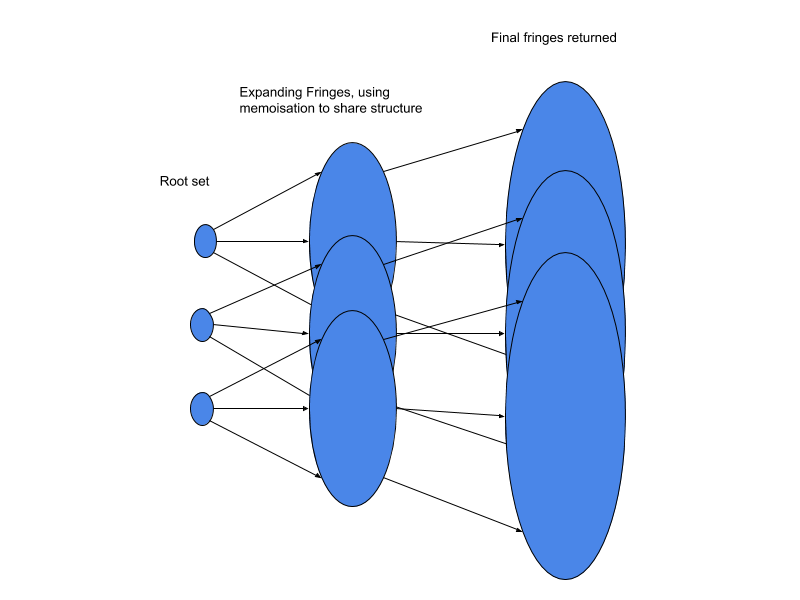
\includegraphics[width=\textwidth]{figs/UptoPairs.png}
  \caption{Execution of an \codeName{Upto} query from multiple roots}
  \label{fig:UptoPairs}
\end{figure}
		
		\paragraph{FixedPoint}
Finally, the FixedPoint take a departure from the parallel implementations above. The reachable set of each node is calculated sequentially using a similar algorithm to above. However the memo now contains all nodes reachable from previously processed roots, allowing for fast convergence of dense graphs.	
	
	\subsection{Pathfinding}
	The \codeName{ShortestPath} and \codeName{AllShortestPaths} commands require us to search a subgraph generated by a relation. Since all edges have unit weight, the pathfinding algorithm reduces to breadth-first-search, which I have implemented in an imperative format while wrapping up error cases in an Either. These functions take, as a parameter, the search step \codeName{ A\ $\Rightarrow$ E \either Set[A]} which represents the edges going out of a node. 
	
	\subsection{Joins}
	The problem of joining two sets of pairs based on shared intermediate values is a requirement for any back-end. 
\[
A\mbox{ }join\mbox{ }B = \setComp{(a, c)}{\exists b. (a, b) \in A \wedge (b, c) \in B}
\]	
I have implemented a simple hash-join\cite{HashJoins}. This operates by first assuming that the size of distinct left-most elements in the right set is smaller than the right-most elements of the left set. Next we build a hash-map index of the right set. We then traverse the left set, looking up right-most-values in the index, to complete the join. An issue with this approach, addressed later, is that we have to build the index upon each \codeName{join} call.

\renewcommand{\baselinestretch}{0.8}
\begin{framed}
\begin{verbatim}
  def joinSet[A, B, C](
      leftRes: Set[(A, B)],
      rightRes: Set[(B, C)]
  ): Set[(A, C)] = {
    // build an index of all 
    // values to join on right, since Proj_B(right)
    // is a subset of Proj_B(Left)
    val collectedRight = mutable.Map[B, mutable.Set[C]]()
    for ((b, c) <- rightRes) {
      val s = collectedRight.getOrElseUpdate(b, mutable.Set())
      s += c
    }
    
    for {
      (left, middle) <- leftRes
      right <- collectedRight.getOrElse(middle, Set[C]())
    } yield (left, right)
  }
\end{verbatim}
\end{framed}
\renewcommand{\baselinestretch}{1.1}

\section{Views and Commits}
In the memory back-end, as will be explained later, views are easy implement as a map of \codeName{ViewId} to \codeName{MemoryTree} and simply updating the \codeName{MemoryTree}, allowing Scala's immutable collections to handle sharing of data in an efficient way. In the other back-ends, backed by non-functional technologies, we need other methods of sharing and inserting to immutable structures. A first observation is that within the operation monad model, each view only has one direct predecessor. We can think of the database as a tree of views with edges representing the successor relation. The path from the root view to a given view can be seen as the operations that generated the view. In this model, if the parent is known, then a child may be defined by the differences between the two. As the database only allows for updates and not deletions, this difference will always be a collection of relations and objects that were added. This collection can be wrapped up in a container called a \codeName{Commit}. At this point, we can disgard the ancestors of a view and see a view as the collection of commits that generated it. This model also allows deletions and overwrites if desired; a commit containing deleted values may be replaced with a new commit which differs only by ot including the deleted values.

\section{Memory Back-end}
The first back-end that I have implemented is a simple, naive memory-based back-end. This back-end follows the denotational semantics, and makes very few attempts to improve performance. This back-end serves as a test-bench back-end, used to create unit tests to test other back-ends. It also allowed me to practice implementation of type erasure and unerasure according to the schema in a controllable environment (that is, without interference from other languages or libraries as in the SQL and LMDB back-ends.)
	\subsection{Table Structure}
	A memory instance stores a concurrent map of \codeName{ViewId} to \codeName{MemoryTree}, which itself is a map of \codeName{TableName} (derived from the \codeName{SchemaDescription}) to \codeName{MemoryTable}. There is a \codeName{MemoryTable} for each object class in the \codeName{SchemaDescription}. A \codeName{MemoryTable} provides lookups using maps for \codeName{DBObjects} and \codeName{Findable}s, in the form of an index to set of objects for each column value. These lookups return objects containing a \codeName{DBObject} and the outgoing and incoming relations for the object, indexed by \codeName{RelationName}. 

\begin{figure}[ht]
\centering
  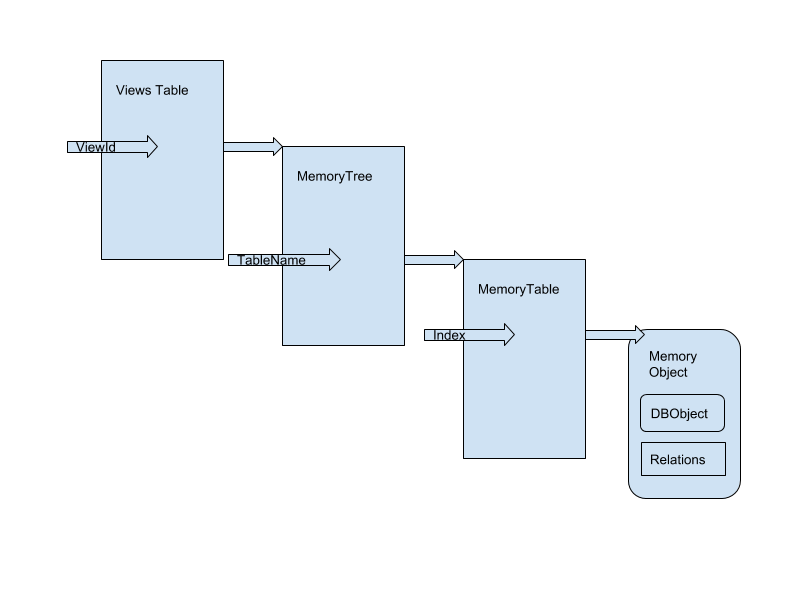
\includegraphics[width=\textwidth]{figs/MemoryHierarchy.png}
  \caption{The lookup procedure for objects in the memory implementation}
  \label{fig:MemoryHierarchy}
\end{figure}

	
	\subsection{Reads}
Reads occur by simply walking over the ADT recursively, following the denotational semantics. The only real departures from the denotational semantics are the left-optimisation (see section \ref{leftOpt}) and use of the generic fixed point algorithms to compute \codeName{Exactly(n, P)}, \codeName{Upto(n, P)}, and \codeName{FixedPoint(P)}. Results are also computed in the \codeName{Either} monad to allow for error checking (for cases such as missing tables). This interpreter can be found in appendix \ref{MemoryInterpreter}.
	
	\subsection{Left Optimisation}\label{leftOpt}
	One of the few optimisations here is the left-optimisation. When we compute the result set of a \codeName{FindPair}, we pass in the subset of left hand side variables we want to compute from. This mostly has an effect when we compute joins (\codeName{Chain}s). Consider joining a query of a few dozen unique right-most values to a large query with several million unique left-most values. The pairs of the right relation only occur in the resulting join if their left-most value is in the set of right-most values of the left relation. Hence pairs which do not have a correct left-most value need not be computed, greatly pruning the search of more complex queries.
\begin{figure}[ht]
	\centering
	\begin{tabular}{p{5cm}p{5cm}p{5cm}}
	\begin{tabular}{|p{1cm}|p{1cm}|}
	    \hline
	    A & B \\ \hline
		1 & 1 \\
		2 & 3 \\ \hline
	\end{tabular} & 	\begin{tabular}{|p{1cm}|p{1cm}|}
		\hline
		B & C \\ \hline
		1 & 4 \\
		2 & 3 \\
		3 & 5 \\
		4 & 6 \\
		7 & 8 \\\hline
		
	\end{tabular} & 	\begin{tabular}{|p{1cm}|p{1cm}|}
		\hline A & C \\ \hline
		1 & 4 \\
		2 & 5 \\ \hline
	\end{tabular} \\
	
	Results of a small query. & A larger query. & Join of the queries.
	\\
     & 	\begin{tabular}{|p{1cm}|p{1cm}|}
		\hline
		B & C \\ \hline
		1 & 4 \\
		3 & 5 \\\hline
		
	\end{tabular} & 	\begin{tabular}{|p{1cm}|p{1cm}|}
		\hline A & C \\ \hline
		1 & 4 \\
		2 & 5 \\ \hline
	\end{tabular} \\
	
	& The large query, left-optimised. & Join of the queries is unaffected.	
	
	\end{tabular}	
	\caption{Joining a large right-hand-side to a small left-hand-side without pruning the search of the right-hand-side results in redundant calculations.}
	\label{fig:LeftHandOptimisation}
\end{figure}
This pattern also makes an appearance in the original LMDB implementation.
	\subsection{Writes}
	Thanks to Scala's immutable collections library, updating the database is fairly easy When inserting a collection of relations, we simply add, relation by relation, each object in the relation, if it does not exist, and update the outgoing and incoming relation map of each object. This update creates new immutable object tables and a new memory tree. This is stored to the map of \codeName{ViewId}  to \codeName{MemoryTree} as a new view.

	\subsection{Storage}
	Objects are stored as \codeName{DBObject}s and their incoming and outgoing relations in wrapper \codeName{MemoryObject}s. \codeName{MemoryObject}s  are hashed and compared by their \codeName{DBObject}s.
	
	\subsection{Mutability}
	The only mutability in the Memory implementation is for the views counter and the views lookup table. Access is kept transactional using a lock.

	\subsection{Pathfinding and fixed point traversal}
	The pathfinding and fixed point traversal methods are simply implemented by calls to the appropriate generic algorithms using the interpreted findPairs function as the search function.


\section{PostgreSQL back-end}
Upon completion of the initial memory back-end, I started work on a PostgreSQL based back-end. This compiles the ADT intermediate representation into SQL queries that are then executed by a Postgres database.

	\subsection{Table Structure}
	The construction of the underlying database uses several SQL tables. These can be partitioned into a set of control tables that will be present in all database instances and a set  of schema defined tables.

		\paragraph{Control Tables}
		\begin{center}
			\begin{tabular}{|p{4cm}||p{4cm}|p{4cm}|} \hline
			Name & Schema & Description \\ \hline
			Default & (ViewId) & Holds the mutable default ViewId \\ \hline
			Commits Registry & (CommitId$^{primary}$, Dummy) & Stores which commits are valid, allows us to give each commit a unique id \\ \hline
			Views Registry & (ViewId$^{primary}$, Dummy) & Stores which views are valid, allows us to give each view a unique id \\ \hline
			Views Table & (ViewId, CommitId) & Stores which commits belong to which view. \\ \hline
			\end{tabular}
		\end{center}
\note{Note: \codeName{ViewId} is a foreign key into the views registry, \codeName{CommitId} is a foreign key into Commits Registry. The Dummy column is needed to fix postgresql syntax when we try to get the next key for a table with one column.}		
		
		\paragraph{Schema defined Tables}
				\paragraph{Control Tables}
		\begin{center}
			\begin{tabular}{|p{4cm}||p{4cm}|p{4cm}|} \hline
			Name & Schema & Description \\ \hline
			Object Table & (ObjectId$^{primary}$, generated) & Generated per schema object in schema description. A schema column is generated per schema object field, with an appropriate SQL type. This allows indexing by findables to get object Ids for queries, and extraction of objects from the database. \\ \hline
			Auxiliary Table & (ObjectId, CommitId) & One auxiliary table is associated with each object table. It stores the object Ids associated with each CommitId, which is a many-many relation \\ \hline
			Relation & (LeftId, CommitId, RightId) & Generated per relation in schema description. Each is associated with a commit.  \\ \hline
			\end{tabular}
		\end{center}
		\note{Note: Object-, Left-, and Right- Ids are foreign keys to the \codeName{ObjectTable}'s ObjectId column.}
	\subsection{Query Structure}
	In order to manage the complexity of queries, I have made use of SQL’s Common Table Expressions feature. CTEs act like let expressions in ML \cite{CTEs}.
	
In this example, I give the compiled result of 
\renewcommand{\baselinestretch}{0.8}
\begin{framed}
\begin{verbatim}
FixedPoint(Rel(Knows))
\end{verbatim}
\end{framed}
\renewcommand{\baselinestretch}{1.1}

	The first CTE used selects all the valid CommitIds.
	
\begin{framed}
\noindent
\textcolor{red}{
\mbox{\texttt{WITH RECURSIVE VIEW_CTE AS }}\\
\mbox{\texttt{~~(SELECT \$commitId FROM \$viewTable WHERE \$viewId = \$id)}}
}
\end{framed}

The next collection of CTEs select the valid instances of each relation from the relation tables.

\begin{framed}
\noindent
\textcolor{blue}{
\mbox{\texttt{WITH	Relation0 AS (SELECT left_id, right_id}}\\
\mbox{\texttt{FROM REL_0_0 JOIN VIEW_CTE ON REL_0_0.CommitId = VIEW_CTE.CommitId)}}
}
\end{framed}

Valid instances are selected from the auxiliary tables to be returned from \mathName{$Id_A$} queries.

\begin{framed}
\noindent
\textcolor{green}{
\mbox{\texttt{AuxTable2 AS (}}\\
\mbox{\texttt{~~SELECT DISTINCT obj_id AS left_id, obj_id AS right_id}}\\
\mbox{\texttt{~~FROM AUXUSERSPACE_People_0 JOIN VIEW_CTE}}\\
\mbox{\texttt{~~ON AUXUSERSPACE_People_0.CommitId = VIEW_CTE.CommitId}}\\
)
}
\end{framed}

CTEs are then created for any repeated subqueries (i.e. those used by \mathName{FixedPoint}, \mathName{Exactly}, and \mathName{Upto})

\begin{framed}
\textcolor{brown}{
\texttt{View1 AS (SELECT * FROM Relation0)}
}
\end{framed}

Repetitive queries are built using inbuilt SQL constructs.
\begin{framed}
\noindent
\textcolor{orange}{
\mbox{\texttt{~~View3 AS (}}\\
\mbox{\texttt{~~~~(SELECT left_id, right_id FROM AuxTable2 )}}\\
\mbox{\texttt{~~~~UNION}}\\
\mbox{\texttt{~~~~SELECT View3.left_id AS left_id, View1.right_id AS right_id}}\\
\mbox{\texttt{~~~~FROM}}\\
\mbox{\texttt{~~~~View3 INNER JOIN View1 ON View3.right_id = View1.left_id}}\\
\mbox{\texttt{~~),}}\\
}
\end{framed}

A CTE is created for the main query, which exposes a \codeName{leftId} and \codeName{rightId}  column

\begin{framed}
\textcolor{cyan}{
\texttt{main_query AS (SELECT left_id, right_id FROM View3 )}
}
\end{framed}

Finally, the main query CTE is joined to fragments which extract the left and rights .
\begin{framed}
\noindent
\mbox{\texttt{(}}\\
\mbox{\texttt{~~SELECT left_table.col_0 AS left_col_0,}}\\
\mbox{\texttt{~~~~~~~~~~right_table.col_0 AS right_col_0}}\\
\mbox{\texttt{~~FROM (}}\\
\mbox{\texttt{~~~~(}}\\
\mbox{\texttt{~~~~~~USERSPACE_People_0 AS left_table}}\\
\mbox{\texttt{~~~~~~JOIN main_query}}\\
\mbox{\texttt{~~~~~~ON left_table.obj_id = main_query.left_id}}\\
\mbox{\texttt{~~~~) JOIN USERSPACE_People_0 AS right_table}}\\
\mbox{\texttt{~~~~ON right_id = right_table.obj_id}}\\
\mbox{\texttt{~~)}}\\
\mbox{\texttt{)}}\\\end{framed}

The \codeName{main} query itself is built compositionally, in that each subquery exposes a \codeName{leftId} and \codeName{rightId},  allowing queries to be composed to form larger queries in a standard form. A full query might look like this:

\begin{framed}
\noindent
\textcolor{red}{
\mbox{\texttt{WITH RECURSIVE}}\\
\mbox{\texttt{~~VIEW_CTE AS (SELECT CommitId FROM VIEWS_TABLE WHERE ViewId = 1),}}\\
}
\textcolor{blue}{
\mbox{\texttt{~~Relation0 AS (SELECT left_id, right_id}}\\
\mbox{\texttt{~~~~FROM REL_0_0 JOIN VIEW_CTE ON REL_0_0.CommitId = VIEW_CTE.CommitId}}\\
\mbox{\texttt{~~),}}\\
}
\textcolor{green}{
\mbox{\texttt{~~AuxTable2 AS (}}\\
\mbox{\texttt{~~~~SELECT DISTINCT obj_id AS left_id, obj_id AS right_id}}\\
\mbox{\texttt{~~~~FROM AUXUSERSPACE_People_0}}\\
\mbox{\texttt{~~~~JOIN VIEW_CTE}}\\
\mbox{\texttt{~~~~ON AUXUSERSPACE_People_0.CommitId = VIEW_CTE.CommitId}}\\
\mbox{\texttt{~~),}}\\}
\textcolor{brown}{
\mbox{\texttt{~~View1 AS (SELECT * FROM Relation0),}}\\
}
\textcolor{orange}{
\mbox{\texttt{~~View3 AS (}}\\
\mbox{\texttt{~~~~(SELECT left_id, right_id FROM AuxTable2 )}}\\
\mbox{\texttt{~~~~UNION}}\\
\mbox{\texttt{~~~~SELECT View3.left_id AS left_id, View1.right_id AS right_id}}\\
\mbox{\texttt{~~~~FROM}}\\
\mbox{\texttt{~~~~View3 INNER JOIN View1 ON View3.right_id = View1.left_id}}\\
\mbox{\texttt{~~),}}\\
}
\textcolor{cyan}{
\mbox{\texttt{~~main_query AS (SELECT left_id, right_id FROM View3 )}}\\
}
\mbox{\texttt{(}}\\
\mbox{\texttt{~~SELECT left_table.col_0 AS left_col_0,}}\\
\mbox{\texttt{~~~~~~~~~~right_table.col_0 AS right_col_0}}\\
\mbox{\texttt{~~FROM (}}\\
\mbox{\texttt{~~~~(}}\\
\mbox{\texttt{~~~~~~USERSPACE_People_0 AS left_table}}\\
\mbox{\texttt{~~~~~~JOIN main_query}}\\
\mbox{\texttt{~~~~~~ON left_table.obj_id = main_query.left_id}}\\
\mbox{\texttt{~~~~) JOIN USERSPACE_People_0 AS right_table}}\\
\mbox{\texttt{~~~~ON right_id = right_table.obj_id}}\\
\mbox{\texttt{~~)}}\\
\mbox{\texttt{)}}\\
	
\end{framed}
	\subsection{Monadic Compilation}
	In order to generate these SQL queries, we need to convert the ADT query to a lower level intermediate representation for each of the SQL fragments to be created. While doing this, we need to gather and rename all of the relation and auxiliary tables that we extract from so that we can form the CTE queries, we also need to find repeated queries to hoist out. In order to do this, we use the monadic compiler pattern described in section \ref{MonadicCompilation}. The compiler state is shown below. When the compilation is complete, depending on the context of the command, we append different extraction queries. For find pairs we need to extract the fields of both the left hand side and the right hand side objects, whereas for pathfinding operations, we only need to extract the \codeName{ObjectId}s along the path as opposed to whole  objects.
	
\renewcommand{\baselinestretch}{0.8}
\begin{framed}
	\begin{verbatim}
case class CompilationContext(
            // Unique identifier for variable names
        varCount: Int,
            // Relations used by the query
        relations: Map[ErasedRelationAttributes, VarName], 
            // tables needed for Findables in the query
        requiredTables: Map[TableName, VarName],
            // the aux (commit) tables needed for the query
        requiredAuxTables: Map[TableName, VarName],
            // Expressions to be repeated over (e.g. by Upto)
        commonSubExpressions: Map[SubExpression, VarName]
)

	\end{verbatim}
\end{framed}
\renewcommand{\baselinestretch}{1.1}

	\subsection{Writes}
	There are several steps in the implementation of writes, though I have not expended  a great deal of effort making them fast. A significant part of this is the "insert or get" SQL query, which looks up an object in the relevant table, returning its \codeName{ObjectId} if it exists and creating the object and returning the new ID if it does not.
	
\begin{framed}
\noindent
\mbox{\texttt{WITH insertOrGetTemp AS (}}\\
\mbox{\texttt{~~INSERT INTO \$objectTable (\$columnNames)}}\\
\mbox{\texttt{~~SELECT \$values WHERE NOT EXISTS (}}\\
\mbox{\texttt{~~~~SELECT 0 FROM }}\\
\mbox{\texttt{~~~~\$objectTable WHERE \$ValueConditions}}\\
\mbox{\texttt{~~) RETURNING \$objId}}\\
\mbox{\texttt{) SELECT * FROM}}\\
\mbox{\texttt{~~insertOrGetTemp  }}\\
\mbox{\texttt{~~~~UNION ALL (}}\\
\mbox{\texttt{~~~~~~SELECT \$objId FROM \$name}}\\
\mbox{\texttt{~~~~~~WHERE \$ValueConditions}}\\
\mbox{\texttt{~~~~)}}\\
\end{framed}
	
	We create a new view and commit, then we run a memoised \codeName{InsertOrGet} over all the leftmost objects to be inserted, then all the right objects to be inserted, yielding tagged relations between \codeName{ObjectIds}. For each inserted relation, the existing relation instances are removed from those to insert, and the remaining inserted to the relevant \codeName{RelationTable} with the correct \codeName{CommitId}. The auxiliary tables are now updated and, on success, the views table is updated.

	\subsection{Mutability}
	As with the memory back-end, all mutability except for the availability of views and the default view is hidden from the user. The SQL back-end uses commits to manage view mutability.
	\subsection{Pathfinding and Fixed Point Traversal}
Pathfinding is implemented by constructing an SQL query to generate right-hand-side \codeName{ObjectIds} for a relation given a left-hand-side \codeName{ObjectId}. This query is used as the search function for the generic pathfinding algorithms. Once paths have been found, their \codeName{ObjectIds} are looked up in the database to find the full values along each path.

Fixed point traversal and repetitions are performed natively in SQL. \codeName{FixedPoint} and \codeName{Upto} are achieved using a recursive CTE, while \codeName{Exactly} is executed by explicitly joining together the required number of repetitions of the sub-relation's query.	

\renewcommand{\baselinestretch}{0.8}
	\begin{framed}
	\begin{verbatim}
	WITH RECURSIVE
    RecursiveCTE AS (
    	(SELECT *, 0 AS Counter FROM BasisCase )
    	UNION
    	SELECT 
    		RecursiveCTE.left_id AS left_id,
    		InductiveCase.right_id AS right_id,
    		Counter + 1 AS Counter
    	FROM RecursiveCTE INNER JOIN InductiveCase
    	ON RecursiveCTE.right_id = InductiveCase.left_id
    	WHERE Counter < Limit
    )
	\end{verbatim}
	\renewcommand{\baselinestretch}{1.1}
	\note{An example of a recursive CTE computing \codeName{Upto}. \codeName{FixedPoint} would omit the counter variable and the limit.}
	\end{framed}
	
	\subsection{Object Storage}
	Objects are stored as in the appropriate \codeName{ObjectTable} in a manner derived from the \codeName{DBObject} of each object. Each \codeName{DBCell} is converted to appropriate SQL type.

\section{LMDB Back-ends}
The final family of back-ends are the LMDB back-ends. LMDB is a lightweight, efficient memory mapped file based Key-Value datastore. \footnote{https://symas.com/lmdb/}.

	\subsection{Common}
	Although I have written several versions of the LMDB back-end, there are several over-arching similarities.
		\paragraph{LMDB API}
			\subparagraph{Terminology}
			LMDB terminology differs slightly from that of more mainstream systems. What would be called a database in SQL is known as an \term{Env} and a table known as a \term{DBI}.
			\subparagraph{Transactions}
				LMDB's transactional model differs from more traditional systems. In short, we need to create a transaction to do read but not write to the database. This stems from LMDB delegating as much work as possible to the OS kernel's memory-mapped file system. All writes are immediately written to the database, whereas starting a read transaction gives a view of the \term{Env} as it was at the start of  the transaction, ensuring that concurrent writes do not affect what is read from the database. Writes may be included in transactions to allow atomic get-and-sets. In practice, the transactions used are very short lived.
			\subparagraph{JVM API}
			The LMDB back-end uses the \codeName{LMDBJava} API \footnote{//github.com/lmdbjava/lmdbjava} to allow access to an LMDB Database from JVM languages (such as Scala). For each \term{DBI}, we have a \codeName{ByteArray} to \codeName{ByteArray} key-value map, much like a \codeName{Map[Array[Byte], Array[Byte]]}.
			
		\paragraph{Storage and Keys}
			In order to write to the database using the LMDBJava API, we need to write the key and value to \codeName{ByteBuffer}s. To generify this process I have introduced two type-classes: \codeName{Keyable} and \codeName{Storable}.
			
\renewcommand{\baselinestretch}{0.8}
\begin{framed}
\begin{verbatim}
trait Keyable[K] { def bytes(k: K): Array[Byte]}

trait Storable[A] {
 def bufferLength(a: A): Int
 final def toBuffer(a: A): ByteBuffer = 
    {/*Allocates a buffer and fills it using declared methods*/}
 def writeToExistingBuffer(a: A, buf: ByteBuffer): Unit
 def fromBuffer(buf: ByteBuffer): LMDBError \/ A
}
\end{verbatim}
\end{framed}	
\renewcommand{\baselinestretch}{1.1}
		
\codeName{Keyable} is a type class which shows that an object can be converted into an array of bytes representing a component of a key. Components may be concatenated to form a key. \codeName{Storable} is a more general type-class that shows that objects can be converted into a \codeName{ByteBuffer}. \codeName{Storable} objects are typically more complex than objects used as keys. Furthermore, a higher marshalling throughput is required for such objects, so a lower-level, \codeName{ByteBuffer} based API is used. Typeclass instances exist to allow sets and lists of \codeName{Storable} objects to be stored.	
			
		\paragraph{Table Structure}
	
 Similarly to the SQL implementation, there are several tables, some generated based on the \codeName{SchemaDescription} and other, control, tables exist regardless. Each table is represented in memory by a subclass of the \codeName{impl.lmdb.common.tables.interfaces.LMDBTable} trait, which provides utility methods such as transactional reads and computations.
 
\begin{center}
	\begin{tabular}{ |p{3cm}||p{3cm}|p{3cm}||p{3cm}|}
 	\hline
 		
	Name & Key Type & Value Type  & Description \\ \hline
	Object Counter & Singleton & ObjId & Atomic counter holds the next ObjectId \\ \hline
	Commit Counter & Singleton & CommitId & Atomic counter holds the next CommitId \\ \hline
	View Counter & Singleton & ViewId & Atomic counter holds the next ViewId \\ \hline
	Default table & Singleton & ViewId & Mutably stores the default view \\ \hline
	Available Views & Singleton & Set[ViewId] & Mutably stores a set of available views \\ \hline
	Views Table & ViewId & List[CommitId] & Maps a view to its constituent commits \\ \hline
	Relations & (ObjectId, CommitId, RelationName) & Set[ObjId] & Single table stores all forward relations in a database \\ \hline
	Reverse Relations & (ObjectId, CommitId, RelationName) & Set[ObjId] & Single table stores the reverse of all relations in the database \\ \hline
	\end{tabular}
\end{center} 
 
 \note{Singleton Keys denote tables with single key.}
 \begin{center}
	\begin{tabular}{ |p{3cm}||p{3cm}|p{3cm}||p{3cm}|}
 	\hline
	Name & Key Type & Value Type  & Description \\ \hline
	Retrieval Table & ObjectId & DBObject & Used to retrieve object data at end of a query \\ \hline
	Empty Index & CommitId & ObjectId & Stores object Ids accessible a view. Used to compute Id_A. \\ \hline
	Column Index &  (Commit, DBCell) & ObjectId & Provides an index over a field of a SchemaObject \\ \hline
	\end{tabular}
\end{center}

For each \codeName{SchemaObject} in the \codeName{Schemadescription}, there exists a \codeName{RetrievalTable}, \codeName{EmptyIndexTable}, and a \codeName{ColumnIndexTable} per column in the \codeName{SchemaObject}.
		
		
		\paragraph{Writes}
		Writes occur in a similar way to the SQL implementation; views are managed using commits. First, we look up all the left- and right-hand-side objects to find their \codeName{ObjectIds}. (If needed, we create new entries in the retrieval table and update the index tables to insert the objects.) We then look up existing instances of the relations for insertion and only write novel ones to the relation table with the new \codeName{CommitId}. Upon success, we create a new view and insert it to the views table and the available views table.

	\subsection{Original LMDB Implementation}
	\note{impl.lmdb.original}

The original LMDB back-end implementation executed queries in much the same way as the in-memory back-end, the only difference being the flat LMDB table structure. Interpretation occurs by a very similar to function that of the memory back-end, instead passing around a list of \codeName{Commit}s to search rather than the memory tree. At the end of a query's execution, the resulting \codeName{ObjectId}s are looked up in the relevant retrieval table to extract the actual objects which are converted into user objects. Pathfinding and the repetition operators are handled in the same way as the memory back-end by calling the relevant generic algorithms.
 

	\subsection{Batched}
	\note{impl.lmdb.fast}
	This is the first variant upon my simple original LMDB back-end, it focuses on making small local optimisations rather than significant algorithmic changes.
	
		\paragraph{Read Batching}
		Firstly, the original implementation made sub-optimal use of LMDB reads. For example, when extracting objects at the end of query execution, it would look up each object individually with its own read transaction. This is sped up by batching together reads from separate keys in the same transaction.
		
		\paragraph{Pre-Caching}
		The result of executing a \codeName{FindSingle} is constant throughout the whole query, so by lifting out and pre-emptively executing any \codeName{FindSingle}s, we speed up execution by removing redundancy. More importantly, this helps enable the next operation.
		
		\paragraph{FindFrom}
		For the pathfinding commands, the transitive queries and \codeName{From} \codeName{FindSingle} query, we are not actually interested in finding all pairs matching the query, but the reachability function \codeName{$A \Rightarrow Set[B]$}. This function forms a kleisli arrow which takes a node and finds its directly reachable neighbours. Since little bookwork is needed to maintain the left hand side of any relation, this greatly simplifies the search. Hence, in these cases, we interpret the query using an alternative interpreter, the \codeName{FindFrom} method. For example, joins now become a concatenation of these arrows (\codeName{flatMap}  in Scala parlance), \codeName{Id} becomes the \mathName{return} function \codeName{($x \Rightarrow Set(x)$)}, \codeName{And}, \codeName{Or}, \codeName{Distinct} all become lower complexity methods, and, finally, we can make use of the \codeName{SimpleFixedPointTraversal} algorithms described in section \ref{SimpleFixedPoint}. The pre-caching in the previous section is useful here, since due to the \codeName{flatMap}s, the computation of \codeName{FindSingle}s would be repeated many times otherwise.

	\subsection{Common Sub-Expression Elimination}
	\note{impl.lmdb.cse}
	A common performance issue in the previous implementation was that of redundant computation and lack of general common sub-expression elimination (CSE). When a common sub-expression is repeated outside of an \codeName{Upto} or \codeName{Exactly} block, then it is recalculated, leading to poor performance. In addition, there is significant redundancy exposed by the above \codeName{FindFrom} optimisation. Consider the calculation of $R join (S join T)$. If a node $n$ appears in the results of $S(m)$, $S(m')$ for distinct $\opRule{(?, m)}{A, B}{R}$, $\opRule{(?, m')}{A, B}{R}$ ($m$, $m'$ are right hand results of R), then $T(n)$ is computed redundantly in the overall calculation. These issues of redundancy can be solved using a combination of global CSE and memoization.

		\paragraph{The Memoisation Problem}
		When looking at a graph data structure, memoization is harder than when looking to optimise pure functions. To optimise a pure function $f\colon A \Rightarrow B$, we only need to store a hash table \codeName{Map[A, B]}. To compute $f(a)$, we simply look up $a$ in the map. If it occurs in the map, we return the mapped value. Otherwise, we call $f$, and insert the result to the map before returning. In a large graph, computing and storing all pairs generated by a query is extremely wasteful, since many of those pairs might never be used (effectively, we would have ignored the left-optimisation). Conversely, memoizing the full left-optimised function, $interpret(Q)\colon Set[A] \Rightarrow Set[(A, B)]$ is also wasteful, since there may be overlap in the sets used as keys. Instead, we memoise the \codeName{FindFrom} function of a query, $findFrom(Q)\colon A \Rightarrow Set[B]$, and reconstruct results from the pairs. This allows for the best overlap. To make the best use of memoization and to avoid over-using memory by memoizing the same query twice, we need to also apply CSE to group together instances of the same sub-query.

		\paragraph{Retrievers}
		A solution to these problems is using an object called a \codeName{Retriever}. This exposes two methods which mirror those from interpreting a query. 
		\renewcommand{\baselinestretch}{0.8}
		\begin{framed}
			\begin{verbatim}
trait RelationRetriever extends Logged {
     def find(from: Set[ObjId]): LMDBEither[Set[(ObjId, ObjId)]]
     def findFrom(from: ObjId): LMDBEither[Set[ObjId]]
}
			\end{verbatim}
		\end{framed}
		\renewcommand{\baselinestretch}{1.1}
		
		For each subquery node in a query(e.g. \mathName{And(Id_A, Or(R_1, R_2 ))}), we generate a retriever. Retrievers for primitive relations (e.g. \mathName{Id_A} , \mathName{Rel(R)}) are un-cached, as LMDB allows for very fast re-computations of these. In the other cases, we use a \codeName{CachedRelationRetriever}, which memorises an underlying lookup function. Using type-enrichment, I have implemented methods such as \codeName{join}, \codeName{and}, \codeName{or}, \codeName{exactly}, \codeName{fixedPoint} on \codeName{RelationRetrievers}, allowing them to be composed analoguously to the query they are generated from. This memoises every node of the query to be executed, yielding a significant reduction of redundancy.
	
		
		\paragraph{Monadic Compilation}
		To avoid storing multiple \codeName{RelationRetriever}s for the same sub-expression, it is useful to reuse the same retriever for every occurrence of a subquery. Hence, an algorithm to construct a query should keep track of previously seen subqueries. This can be achieved using the monadic compilation pattern (Section \ref{MonadicCompilation}). The compilation state stores a hashmap of all the subtrees that have already been computed (Similarly to constructing a binary decision diagram in automated theorem proving). 
		
\renewcommand{\baselinestretch}{0.8}
\begin{framed}
\begin{verbatim}
class QueryMemo(
    val pairs: Map[UnsafeFindPair, RelationRetriever], 
    val singles: Map[UnsafeFindSingle, SingleRetriever]
)
\end{verbatim}
\note{Compilation state}
\end{framed}
\renewcommand{\baselinestretch}{1.1}

		The compilation function checks the memo for a precomputed retriever for a query. If a matching retriever is not found, it recurses to compute and compose subtree results to produce a new retriever. The new retriever is added to the compilation state.
		
	\subsection{Complex Common sub-expression Elimination}
	\note{impl.lmdb.fastjoins}
Despite these optimisations, there are still sources of redundancy.

		\paragraph{Index Building}
			Firstly, the original CSE implementation uses the excessively generic \codeName{joinSet} function to join result sets. This function wastes time by computing an index on every call. Instead, we can change the definition of a \codeName{Retriever}'s public interface to mitigate the need to build indices.
			\renewcommand{\baselinestretch}{0.8}
			\begin{framed}
			\begin{verbatim}
			trait RelationRetriever extends Logged {
  def find(from: Set[ObjId]): LMDBEither[Map[ObjId, Set[ObjId]]]
  def findFrom(from: ObjId): LMDBEither[Set[ObjId]]
}
			\end{verbatim}
			\end{framed}
			\renewcommand{\baselinestretch}{1.1}
			Indeed, the function to join a pair of retrievers becomes a simpler \codeName{flatmap} of one map to another. Functions such as the \codeName{union} and \codeName{intersection} of retrievers also become simpler. (\note{See impl.lmdb.fastjoins.retrievers.RelationRetriever.RelationRetrieverOps})

		\paragraph{Exactly}
		This implementation also explores other formulations of the \mathName{Exactly(n, P)} query. \codeName{Exactly} effectively joins together \mathName{n} repetitions of the underlying query in a sequential fashion. Despite making good reuse of the query \codeName{P}, this fails to memoise the repetition of the \mathName{join}; each \mathName{join} has different input subqueries, so it cannot be memoised.
		

\begin{figure}[ht]
\centering
  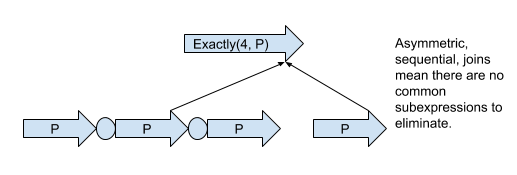
\includegraphics[width=\textwidth]{figs/SequentialJoins.png}
  \caption{Sequential joins provide little common substructure to eliminate.}
  \label{fig:SequentialJoins}
\end{figure}
		
		
		As joins over the set of results of subqueries form a \mathName{Monoid} (proven in appendix \ref{MonoidJoins}), we associatively reorder the evaluation of \mathName{joins}, aiming for as much common substructure as possible. This can be performed in a manner similar to square-and-multiply exponentiation.

We calculate retrievers for $P^{2^i}$ for each $i$ less than the bitlength of $n$. We then join the relevant retrievers to to get a retriever for $P^n$. This only uses $O(Log_2(n))$ distinct joins, and makes very good reuse of the join functions. 

\begin{figure}[ht]
\centering
  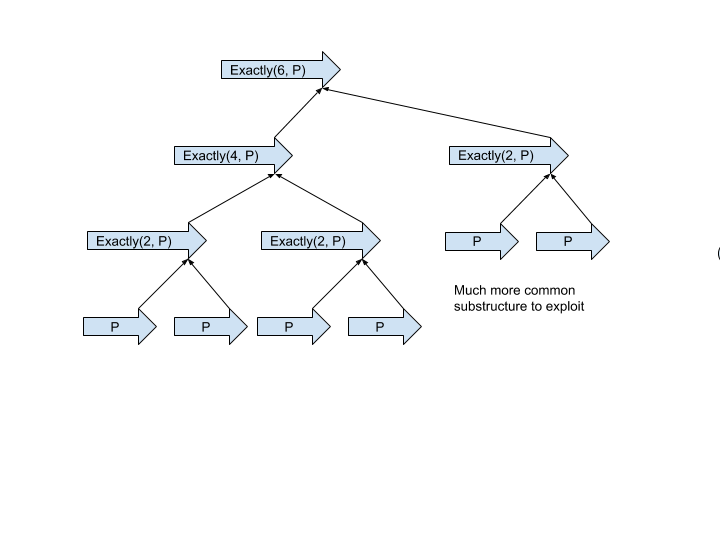
\includegraphics[width=\textwidth]{figs/CommonJoins.png}
  \caption{By reordering joins, we gain significant common substructure to eliminate.}
  \label{fig:CommonJoins}
\end{figure}

\renewcommand{\baselinestretch}{0.8}
\begin{framed}
\begin{verbatim}
def exactly(n: Int): RelationRetriever = repeat(n, outer, IdRetriever)

private def repeat(
  n: Int,
  acc: RelationRetriever,
  res: RelationRetriever
): RelationRetriever = if (n > 0) {
  val newRes = if((n & 1) == 1)  (res join acc) else res
  val newAcc = acc join acc
  repeat(n >> 1, newAcc, newRes)
} else res
\end{verbatim}
\end{framed}
\renewcommand{\baselinestretch}{1.1}

		\paragraph{Upto Optimisation}
			We can also re-formulate an \mathName{Upto(n, P)} as an \mathName{$Exactly(n, Or(P, Id_A))$}. (As proven in appendix \ref{UptoOpt}.) We can hence use the same optimisation as above on \mathName{Upto}. We cannot, however produce a similar static formulation for \codeName{FixedPoint} as we cannot tractably predict when it will converge.
			
			\renewcommand{\baselinestretch}{0.8}
			\begin{framed}
			\begin{verbatim}			
    def upto(n: Int): RelationRetriever =
        repeat(n, outer or IdRetriever, IdRetriever)
			\end{verbatim}
			\end{framed}
			\renewcommand{\baselinestretch}{1.1}

\section{Summary}
This chapter has explained overarching programming techniques and how back-ends were constructed. Furthermore it introduces several optimisations to LMDB back-ends. The first is the simple left-optimisation which prunes search trees for queries which match a small proportion of the graph. The second is elementary CSE-elimination which we expect to provide a speed up over queries with common sub-structure. Finally there is the \codeName{Exactly} and \codeName{Upto} reformulation which ought to improve performance over transitive queries.

\chapter{Evaluation}
\section{Unit Tests}
The correctness of each back-end is tested using a suite of 45 unit tests which verify adherence to the specified semantics. These have  wide range, testing over all the commands, all the possible ADT nodes, and the correct usage and separation of views. I have been using the regression test model, in that discovering a non-trivial bug, I've written a test case to target that bug, ensuring that it is not leaked into production again. These tests provide good evidence that all the implemented back-ends are correct in the small.
\section{Performance Tests}
	In order to evaluate the effectiveness of the various optimisations to the LMDB back-ends described above, it was necessary to run performance tests over wide range of queries. The various LMDB back-ends were tested against each other as a control and particularly against the SQL back-end as a standard to beat. The in-memory back-end was omitted as initial tests indicated that it runs with approximately the same algorithmic characteristics as the Original LMDB implementation, which shares the same interpreter model. The LMDB implementation was able to index faster than Scala's tree based hash maps, which are used by the in-memory implementation. Furthermore, the original LMDB implementation is typically around 3x slower than the batched version across a most tests, since a majority of the algorithms it uses for interpretation are the same.
	\subsection{Hardware}
	Tests were run on the oslo machine belonging to Timothy Jones' group. Its specifications are shown below. All of the back-ends ran off of an SSD.
\\\\	\begin{tabular}{|p{5cm}p{10cm}|}
	\hline
		Processor : & 2x OPTERON 16-CORE 6376 \\
		Memory : & 8x 16G DDR3 1600 ECC Reg Server memory\\
	\hline
	\end{tabular}
	\subsection{Datasets}
	To evaluate tests on non-trivial examples, I sought to construct datasets over which large queries were feasible.

		\paragraph{IMDB and TMDB}
		The first and most used collection of tests are derived from the TMDB movie database,the most popular 5000 of which were collected from kaggle \cite{TMDB5000}

The CSV data was processed using a python script into a simplified JSON format. A separate, larger dataset derived from IMDB was constructed from tests for another graph database \cite{IMDB} and manually (in python) converted to the same JSON format. I then wrote a Scala script which reads the JSON and writes the relations to a given database instance.

Slightly different parameters were given when generating each dataset.

\begin{center}
	\begin{tabular}{ |p{3cm}||p{3cm}|p{3cm}||p{3cm}|  }	
	\hline
        Name & Movies Size & People Size & Notes \\ \hline
        smallest & 100 & 10351 & 100 movies with most actors \\ \hline
        small & 250 & 18167 & 250 movies with most actors \\ \hline
        small _sparse & 250 & 1029 & 250 movies with fewest actors \\ \hline
        medium & 1000 & 35626 & 1000 movies with most actors \\ \hline
        medium_sparse & 1000 & 6310 & 1000 movies with fewest actors \\ \hline 
       large & 12862 & 50134 & Largest dataset \\ \hline
	\end{tabular}
\end{center}

The objects in the database are as follows:
\paragraph{Objects}
\begin{center}
	\begin{tabular}{ |p{3cm}| p{3cm}|}
	\hline
	Name & Fields \\ \hline
	Person & Name: String \\ \hline
	Movie & Name: String Language: String \\ \hline
	Date & Time: Long \\ \hline
	Place & Place: String \\ \hline
	Genre &	Genre: String \\ \hline
	\end{tabular}
\end{center}

\paragraph{Relations}
\begin{center}
	\begin{tabular}{ |p{3cm}|| p{3cm}| p{3cm}|}
	\hline
		Name &  From & To \\ \hline
		ActsIn & Person & Movie \\ \hline
		Directed & Person & Movie\\ \hline
		HasBirthday &Person & Date\\ \hline
		BornIn & Person & Place\\ \hline
		HasGenre & Movie & Genre\\ \hline
	\end{tabular}
\end{center}

		\paragraph{UFC}
		
		A second dataset, built from UFC fight data \cite{UFC}, was constructed in the same way to produce one JSON dataset.
		
		\paragraph{Objects}
\begin{center}
	\begin{tabular}{ |p{3cm}| p{9cm}|}
	\hline
		Name & Fields \\ \hline
		Person & Name: String, Height: Int, Weight: Int\\ \hline
	\end{tabular}
\end{center}

\paragraph{Relations}
\begin{center}
	\begin{tabular}{ |p{3cm}|| p{2cm}| p{2cm}||p{3cm}|}
	\hline
		Name &  From & To & notes \\ \hline
		Beat & Person & Person & \\ \hline
		ShorterThan &  Person & Person & Transitive reduction of the shorter than relation \\ \hline
		LighterThan & Person & Person & Transitive reduction of the lighter than relation \\ \hline

	\end{tabular}
\end{center}
		
		The \codeName{ShorterThan} and \codeName{LighterThan} relations produce extremely sparse graphs which take a long time to converge under transitive closure. The graph has 1562 nodes and 3571 \codeName{Beat} relations.
	\subsection{Test Harness}
	In order to run tests against each other, I have written a typesafe test harness to run on oslo. This standardises the interface that individual benchmark instances must implement. Each test must provide  \codeName{setup} and \codeName{test} methods which take a \codeName{DBInstance} parameter. The test method is further enumerated by a \codeName{TestIndex}. The test specification must give a maximum index and a mask to avoid running inappropriate back-ends, such as those that might take too long on a large data-set. The benchmarks that I have run test only the read speed; the time taken to construct the database is not included. Finally, the test harness compares the hash of the result of each query with that produced by the reference implementation, hence verifying that all implementations produce the same result. This provides good evidence that the implementations follow the same specified semantics.
	
	\subsection{Results}
		\paragraph{Overall Picture}
		An overall view of the results is that, as might be expected, the SQL implementation is the fastest over short, indexing heavy, queries. The most aggressively optimised LMDB implementation typically performing slightly worse than those with fewer optimisations over these queries. This likely due to the overheads of generating the memo. However, when longer graph queries expose the redundancies noted in the preceding sections, speed ups of orders of magnitude can be seen over both the other LMDB implementations and over SQL. This can particularly be seen in the cases of \codeName{FindPair} transitive queries.

		A point to note is that I am ignoring evaluation of pathfinding queries. For simplicity, the pathfinding implementation re-evaluates the underlying step function query at each stage of the breadth first search. This seems to particularly punish the SQL implementation, to the extent that it is around 2000x slower than the LMDB reference implementation. Stateful solutions to speed this up might include creating a temporary table in the database to store the subgraph being searched. However, this would complicate the SQL implementation, since clearing up on error would require validating state. Hence, I am ignoring the pathfinding tests for the purpose of back-end comparison.
		As the differences in performance due to the features of different back-ends are relatively large and benchmarks test over a range of queries, I have ommitted error bars in performance result graphs.


\paragraph{Redundancy}
This first test demonstrates the removal of redundancies in \codeName{FindSingle} commands. There is clearly a major increase in speed due to the introduction of CSE and memoisation. Since this is a \codeName{FindSingle} query, there is no usage of the optimised join formulations, so there is no speed gain by the most optimised LMDB back-end. Postgres fails to fully optimise away the redundancy, even with use of the \texttt{DISTINCT} modifier of queries, Hence it ends up running out of temporary disk space on this query. Results can be seen in figure \ref{fig:RedundancyResult}.
				
\resultTable{Redundancy}{4 each}{
\texttt{KevinBacon >> coactor;}\\\\
\texttt{KevinBacon >> (coactor -->--> (}\\
\texttt{coactor -->--> coactor));}\\\\
\texttt{KevinBacon >> (coactor -->--> ( }\\
\texttt{coactor -->--> (coactor -->--> 	coactor)));}\\\\

Where

\texttt{def coactor = ActsIn --><-- ActsIn}

\\Finds increasing order co-actors with Kevin Bacon
}{ \reference   	& 	381,972 & 1\\
 \cse 			&   379,280 & 0.993 \\
 \batched 		&	9,318,741 & 24.4 \\
 \postgres    	&	Did not finish & Did not finish \\
} 

\begin{figure}[ht]
\centering
  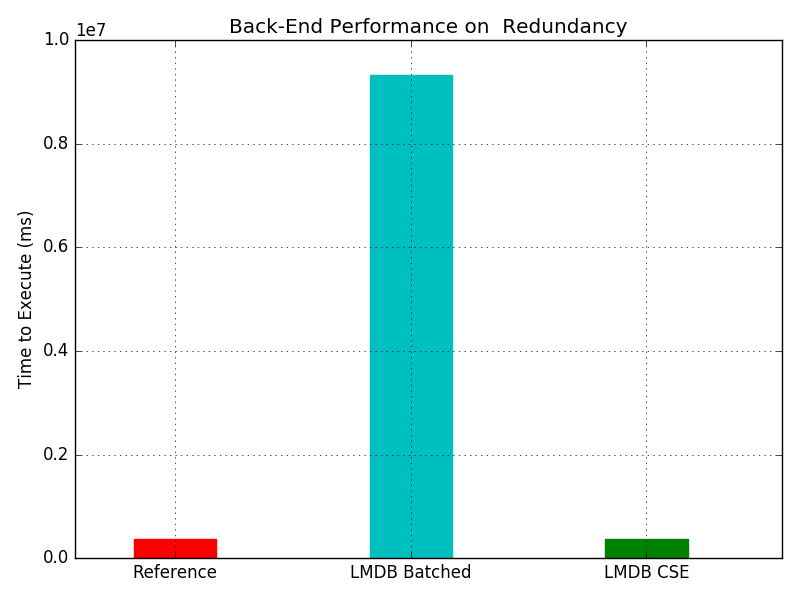
\includegraphics[width=0.9\textwidth]{scripts/Redundancy.png}
  \caption{Read performance for redundancy queries}
  \label{fig:RedundancyResult}
\end{figure}

		\paragraph{Intersections and Unions}
	These two tests make use of the \mathName{And} and  \mathName{Or} operators to combine several subqueries with some underlying common structure. Both resulted in similar performance patterns. The Postgres implementation comfortably outperformed all LMDB implementations across this index-heavy test, while the CSE related optimisations appeared to add overheads greater than the redundancy they removed. I expect the reasons for this are that the redundancy exposed by the underlying sub queries is limited and that the implementation of unions and intersection in Scala sets is slower than the optimised C implementation used by Postgres. In addition, constructing an intersection and union over the memoisation in the LMDB implementation also adds some overhead and reduces locality of reference.	Results can be seen in figures \ref{fig:IntersectionResults} and \ref{fig:UnionResults}.

\resultTable{Intersections}{40 each}{
\texttt{(coactorWith(KevinBacon));}\\\\
\texttt{(coactorWith(KevinBacon) \& coactorWith(TomCruise));}\\\\
\texttt{(coactorWith(KevinBacon) \& coactorWith(TomCruise) \& }\\\texttt{coactorWith(TomHanks));}\\\\
Where\\
\texttt{def coactorWith(a: Person) = }\\
\texttt{ActsIn --> (a >> ActsIn) <-- ActsIn} \\

\codeName{CoactorWith(a)} defines a relation between actors who are 
\\ coactors in a movie that \codeName{a} also acted in.
}{ 
 \reference 			&   879,984 & 1 \\
 \cse 					&	827,734 & 0.941	\\
 \batched 				&   791,678 & 0.900 \\
 \postgres    			&	106,165 & 0.121 \\
}
\begin{figure}[ht]
\centering
  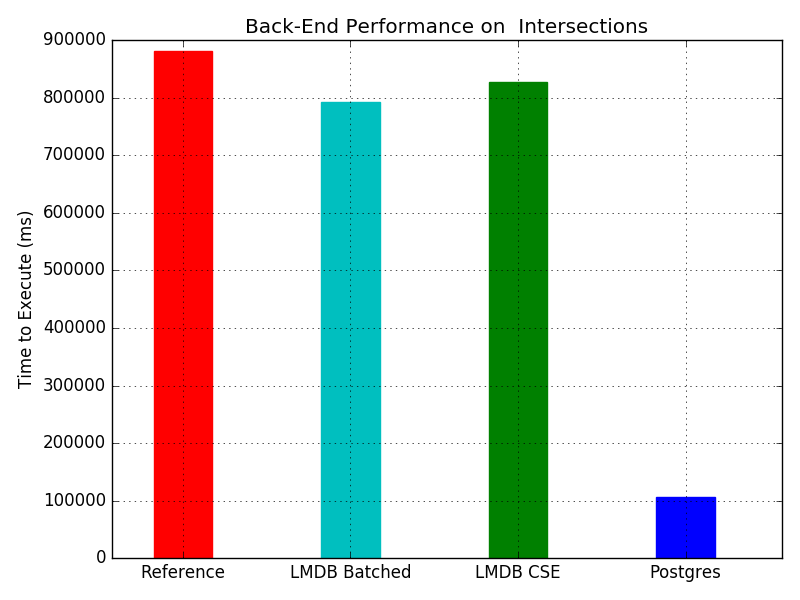
\includegraphics[width=0.9\textwidth]{scripts/Intersections.png}
  \caption{Read performance for intersection queries}
  \label{fig:IntersectionResults}
\end{figure}

					\resultTable{Unions}{40 each}{\texttt{(coactorWith(KevinBacon));} \\\\
\texttt{(coactorWith(KevinBacon) | coactorWith(TomCruise));}\\\\
\texttt{(coactorWith(KevinBacon) | coactorWith(TomCruise) |}\\\texttt{coactorWith(TomHanks));}\\\\
Where\\
\texttt{def coactorWith(a: Person) = }\\ 
\texttt{ActsIn --> (a >> ActsIn) <-- ActsIn} \\
}{ 
 \reference 			&   853,664 & 1 \\
 \cse 					&	824,799 & 0.966	\\
 \batched				&   800,455 & 0.938 \\
 \postgres    			&	112,488 & 0.132 \\
 }	
 
 \begin{figure}[ht]
\centering
  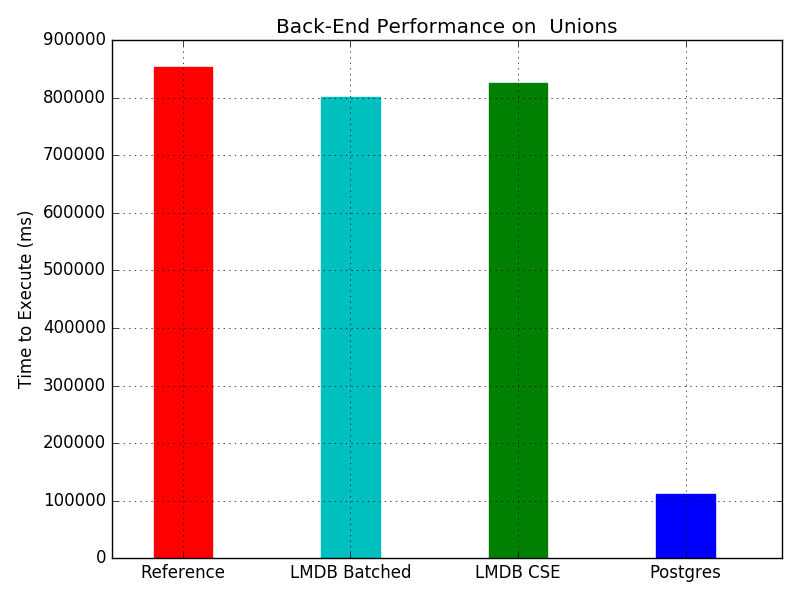
\includegraphics[width=0.9\textwidth]{scripts/Unions.png}
  \caption{Read performance for union queries}
  \label{fig:UnionResults}
\end{figure}

		\paragraph{Tests that involve repetitions}
		These are a suite of benchmarks for testing the optimisations and performance on repetitive queries. A general overview is that the join-reordering optimisations strongly sped up benchmarks which ran \codeName{FindPair} queries. However, in \codeName{FindSingle} queries this formulation did not compete as strongly with the fast \codeName{SimpleFixedPointTraversal} methods. SQL performed strongly in \mathName{Upto} queries which use built in, optimised, recursive CTEs to calculate results, but less strongly in \mathName{Exactly} queries which do not have a built-in formulation.

			\subparagraph{Exactly Test}
			This test runs \codeName{FindSingle} \mathName{Exactly} queries of varying lengths over the small movies database. As explained, the \codeName{SimpleFixedPointTraversal} \codeName{exactly} method is faster than any gains by the join reordering in the mpst optimised LMDB version. Postgres also performed poorly due to the lack of a recursive CTE for self joins. See figures \ref{fig:ExactlyResults} and \ref{fig:ExactlyTestLog}.
	\resultTable{Exactly}{50}{
	\texttt{TomHanks >> (}\\
	\texttt{((ActsIn -->(KevinBacon >> ActsIn))<-- ActsIn) * (index.i \% 10);}	\\
	\texttt{)}
	
\\Finds higher order coactors of Tom Cruise over the subgraph
\\of movies acted in by Kevin Bacon
}{ 
 \reference 			&  	1,752 	& 1 \\
 \cse 					&	1,798 	& 1.03	\\
 \batched				&   1,513 	& 0.834 \\
 \postgres    			&	102,461 & 58.5 \\
 }
 
 \begin{figure}[ht]
\centering
  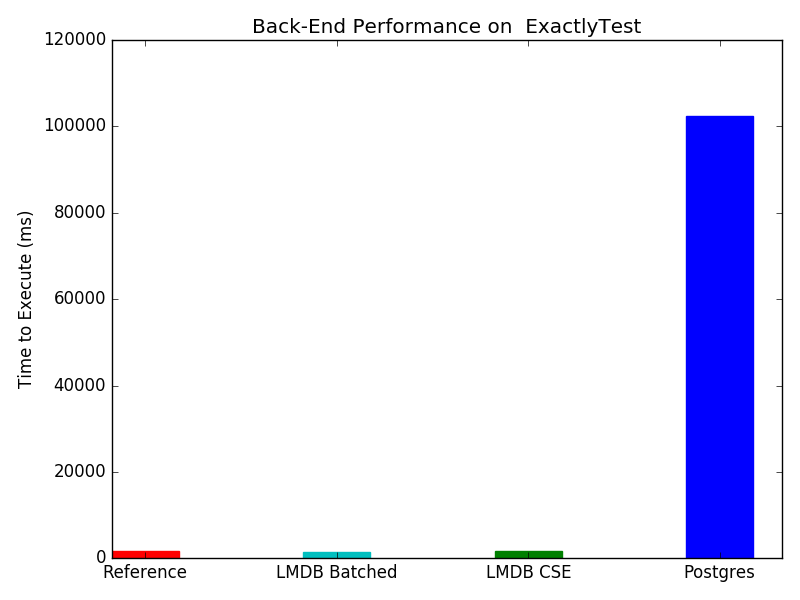
\includegraphics[width=0.9\textwidth]{scripts/ExactlyTest.png}
  \caption{Read performance for \codeName{Exactly} queries}
  \label{fig:ExactlyResults}
\end{figure}

 \begin{figure}[ht]
\centering
  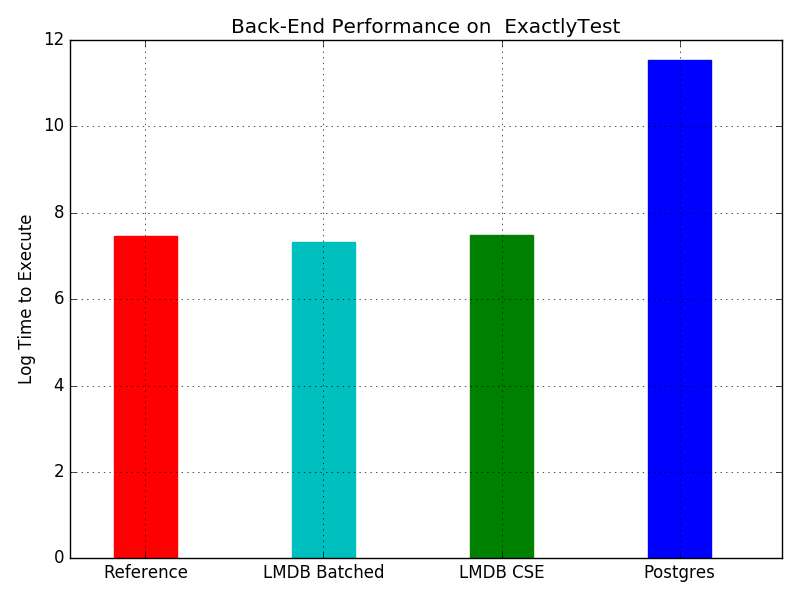
\includegraphics[width=0.9\textwidth]{scripts/ExactlyTestLog.png}
  \caption{Log-Read performance for \codeName{Exactly} queries}
  \label{fig:ExactlyTestLog}
\end{figure}
			\subparagraph{Exactly Pairs}
This test instead runs a \codeName{FindPair}, variable-length \mathName{Exactly} query over the small movies database. Since this test involves bookkeeping of the root for each pair found, the \mathName{Exactly}-optimised LMDB implementation significantly outperforms the other LMDB implementations which use the generic algorithm. Postgres also performs well in this test, showing minimal slowdown from the \codeName{FindSingle}queries. The LMDB implementations, however, do experience a slowdown from \codeName{FindPair}. See figure \ref{fig:ExactlyPairsResults}.
	\resultTable{ExactlyPairs}{50}{
	\texttt{((ActsIn -->(KevinBacon >> ActsIn))<-- ActsIn) * (index.i \% 10));}

\\Finds higher order pairs of coactors over the subgraph
\\of movies acted in by Kevin Bacon	
	}{ 
 \reference 			&  	83,269 		& 1 \\
 \cse 					&	1,792,388 	& 21.5 \\
 \batched				&   1,787,390 	& 21.5 \\
 \postgres    			&	107,797 	& 1.29 \\
 }	

\begin{figure}[ht]
\centering
  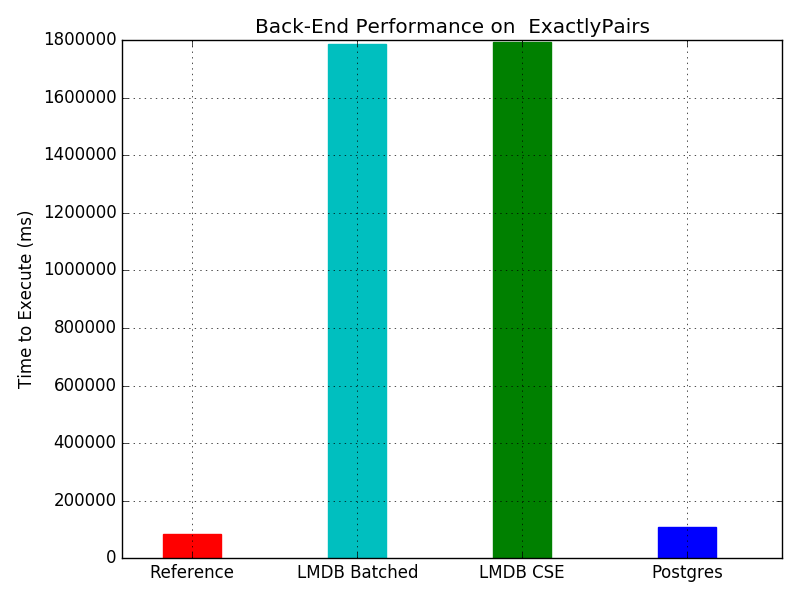
\includegraphics[width= 0.9 \textwidth]{scripts/ExactlyPairs.png}
  \caption{Read performance for exactly \codeName{FindPair} queries}
  \label{fig:ExactlyPairsResults}
\end{figure}

			\subparagraph{UptoTest}
				This test runs \mathName{Upto} based \codeName{FindPair} queries over the large IMDB database. Here the upto-optimisation of the final LMDB back-end provides a significant speed-up, such as 225x on the other LMDB back-ends and 1.5x over Postgres. See figure \ref{fig:UptoTestResult}.
				\resultTable{Upto}{10}{
				\texttt{((ActsIn -->(KevinBacon >> ActsIn))<-- ActsIn).*(}\\
				\texttt{0 --> index.i);}
				
\\Finds actors linked by up to \mathName{i} insances of the coactor 
\\relationship in the subgraph of movies acted in by Kevin Bacon
}{ 
 \reference 			&  	126,448 	& 1 \\
 \cse 					&	28,491,910 	& 225 \\
 \batched				&   28,423,658 	& 225 \\
 \postgres    			&	197,880 	& 1.56 \\
 }	
 
\begin{figure}[ht]
\centering
  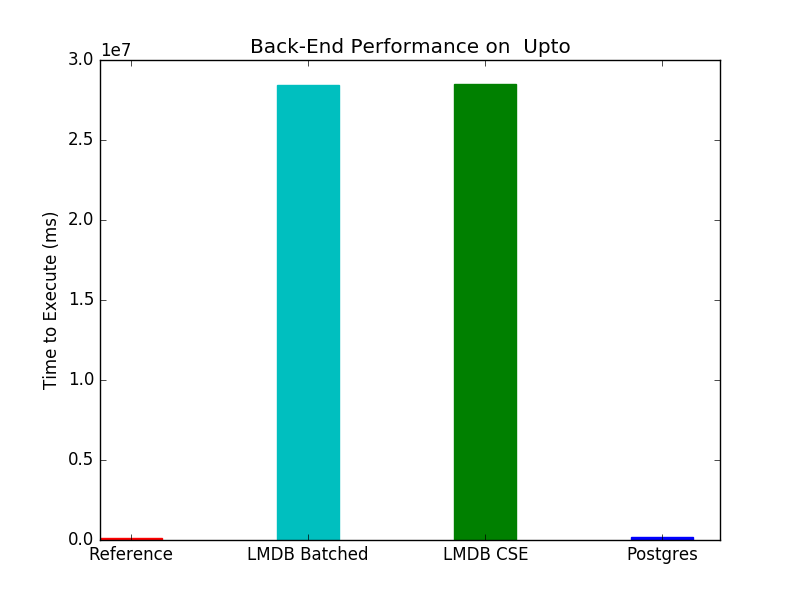
\includegraphics[width=0.9\textwidth]{scripts/Upto.png}
  \caption{Read performance for \codeName{Upto} queries}
  \label{fig:UptoTestResult}
\end{figure}

 \begin{figure}[ht]
\centering
  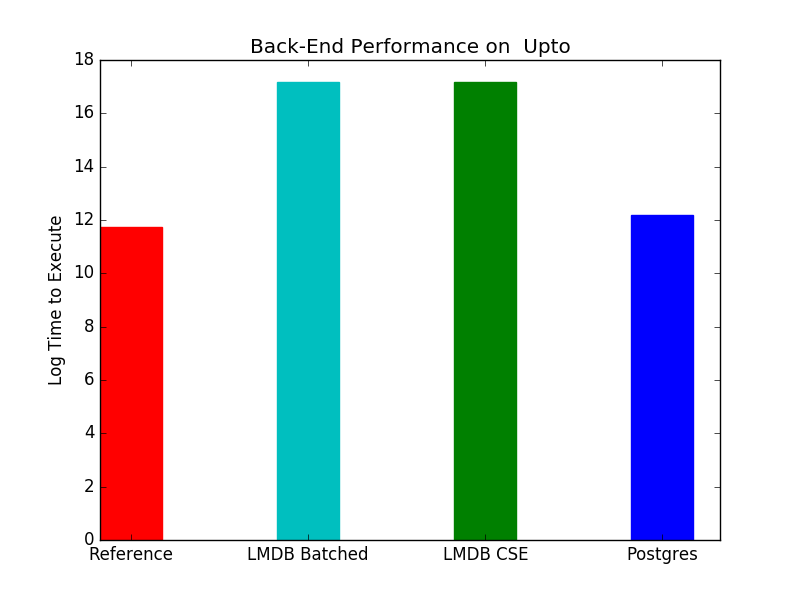
\includegraphics[width=0.9\textwidth]{scripts/UptoLog.png}
  \caption{Log-Read performance for \codeName{Upto} queries}
  \label{fig:UptoLogResult}
\end{figure}
			\subparagraph{UptoLarge}
			
				Since the more naive LMDB instances took seven hours each to complete the above test, I re-ran the benchmark for only the reference and Postgres implementations for a longer period of time, yielding a similar ratio of performance. These results can be seen in figure \ref{fig:UptoLargeResults}.
				\resultTable{Upto}{100}{
				\texttt{((ActsIn -->(KevinBacon >> ActsIn))<-- ActsIn).*(}\\
				\texttt{0 --> (index.i \% 10)}\\
				\texttt{);}}{ 
 \reference 			&  	1,059,091 	& 1 \\
 \postgres    			&	1,557,314 	& 1.47 \\
 }
 
 \begin{figure}[ht]
\centering
  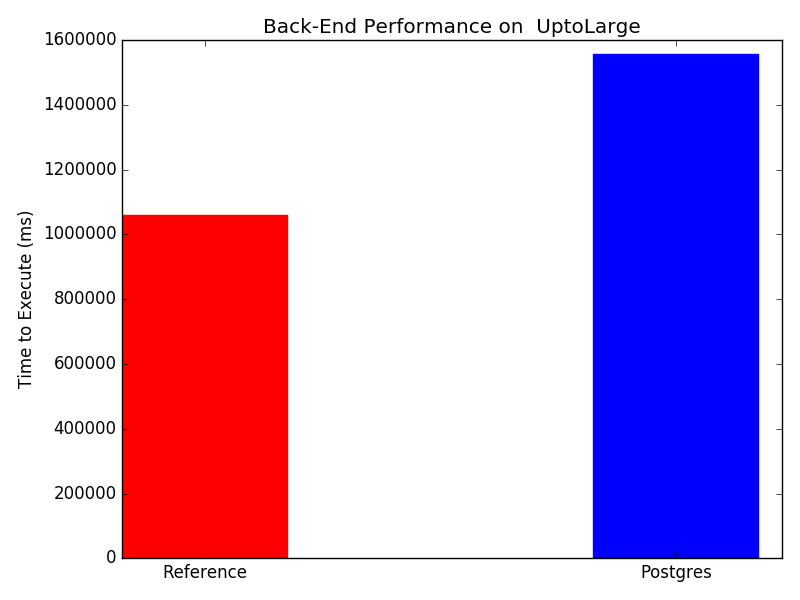
\includegraphics[width=0.9\textwidth]{scripts/UptoLarge.png}
  \caption{Read performance for large \codeName{Upto} queries}
  \label{fig:UptoLargeResults}
\end{figure}
	
			\paragraph{JoinSpeed}
				This test is  to demonstrate the cost of joins. We interleave queries that calculate two subqueries and then combine them. For half of the queries, the \codeName{And} operator is used, which is assumed to be fast. For the other half, a \codeName{Chain} is used. In theory, the difference between these two types of queries should give us an idea of the cost of a join, as seen in figure \ref{fig:JoinSpeedResults}.
			\jsTable{Join Speed}{150 each}{
			\texttt{(ActsIn --><-- ActsIn) \& (ActsIn --><-- ActsIn);}\\\\
\texttt{(ActsIn --><-- ActsIn) -->--> (ActsIn --><-- ActsIn);}
			}{
			\reference   	& 	633 & 1,443 & 2.28 	\\
 			\cse 			&   884 & 2,285 & 2.58   	\\
			\batched 		&	953 & 2,028 & 2.12	\\
			\postgres    	&	345 & 1,557 & 4.51	\\}
			
\begin{figure}[ht]
\centering
  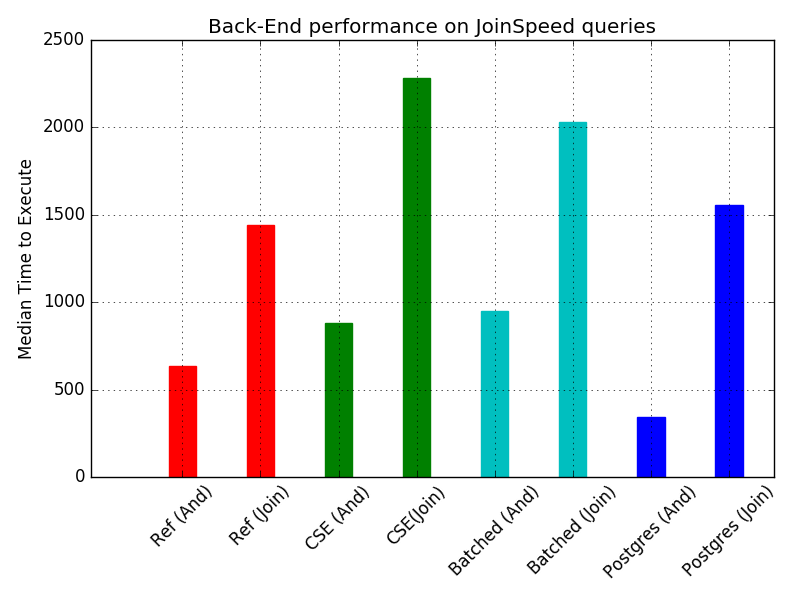
\includegraphics[width=0.9\textwidth]{scripts/joinspeedComp.png}
  \caption{Overall read performance for Join-Speed queries}
  \label{fig:JoinSpeedResults}
\end{figure}
There are some things to note from these figures. Firstly, around 7\% of the LMDB times are consistently around 1000-2000ms larger than the rest of the values. This can be seen in figure \ref{fig:LatencyDensity}. I have yet been unable to determine if this is is due to the LMDB datastore itself or if there is another background task interfering. As a result of this bimodal distribution, erroneously large standard deviation values occured. Hence, I have used the median latencies of queries instead of mean. The data suggests that Postgres can execute index and intersection queries very quickly but suffers when join queries are used. The join-optimised LMDB implementation shows itself again to be the best at removing redundancy among the LMDB implementations.

\begin{figure}[ht]
\centering
  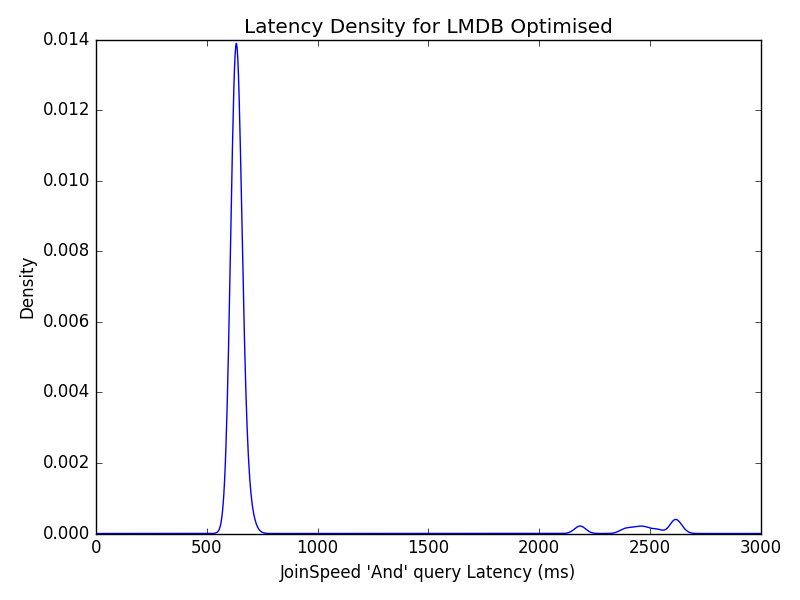
\includegraphics[width=0.9\textwidth]{scripts/LatencyDensity.png}
  \caption{The distribution of values for the \mathName{And} query of JoinSpeed. Around 7\% of values fall into the density on the right of the graph. }
  \label{fig:LatencyDensity}
\end{figure}


			\paragraph{Closing Thoughts}
			These benchmarks provide some insights into the strengths and weaknesses of the various optimisations I have written. The results lend themselves to the idea of constructing an adaptive back-end that chooses its interpretation strategy based on heuristics of the performance of given queries. These performance statistics also show that specialised graph engines can easily outstrip the performance of generalised relational databases over particular queries within the domain.


	
\chapter{Conclusion}

\section{Successes}
To the best of my knowledge, the graph database system I have built over the last seven months is one of the, if not the, first explicitly purely functional graph database systems in existence. This project is a demonstration that complex, performant software projects can be built using purely functional languages, whilst keeping the benefits of strong type systems. I feel that despite having written the project in Scala, a high level, often inefficient language I have achieved an acceptable level of performance for graph traversal. Although the system would need significant work in the areas of security, networked access, and tuning to real-world use cases to become commercially viable, it stands as a solid prototype for potential future systems.

\section{Further extensions}
Interesting extensions to the core project that, given more time, I would have been interested to explore include
\begin{itemize}
 \item An increase in the use of laziness to allow larger queries over larger graphs. Currently, the size of queries are limited by how large the result sets of sub-queries. However, the Postgres implementation typically runs out of temporary file space before this happens.
 \item The implementation of deletions and garbage collection of unused views in the database. Garbage collection in particular might be difficult, as the database is not required to store any state about client instances.
 \item Exploration of  improvement of the schema system using a dependent types library, such as shapeless.
 \item Rewriting the lowest layer of the LMDB back-ends' interpreters in C or another low level language to extract maximum performance from the LMDB system, without having to construct Scala collections at every step.
\end{itemize}

\section{Lessons learned}
	With hindsight, I might have aimed to build a narrower project, focusing on a single back-end and comparing  performance against a widely used graph database such as Neo4j. Although I very much enjoyed the chance to build a large project in a purely functional style, implementing the large number of moving parts in the project distracted from implementing more interesting optimisations and truly digging down to exploit all redundancy.

\section{Concluding Thoughts}
I hope for another chance to explore this space as I feel there are still many areas worth investigating.




%%%%%%%%%%%%%%%%%%%%%%%%%%%%%%%%%%%%%%%%%%%%%%%%%%%%%%%%%%%%%%%%%%%%%
% the bibliography
\addcontentsline{toc}{chapter}{Bibliography}
\bibliography{diss}

%%%%%%%%%%%%%%%%%%%%%%%%%%%%%%%%%%%%%%%%%%%%%%%%%%%%%%%%%%%%%%%%%%%%%
% the appendices
\appendix
\addcontentsline{toc}{chapter}{Appendix}
\chapter{The Domain \clos}

For the various semantics proofs it is necessary to define the Scott domain $\clos$ for some object type $A$ and $View_{\Sigma}$ $v$. This domain is the set of subsets $x$ such that $\deno{Id_A} \subseteq x \subseteq A \times A$ with bottom element $\bot = \deno{Id_A}$ and partial order $x \sqsubseteq y \Leftrightarrow x \subseteq y$. From this point on, I shall use $x \subseteq y$ to mean $y \sqsubseteq x$.

\hfill\begin{minipage}{\dimexpr\textwidth-1cm}
\paragraph{$\clos$ is a domain}


Firstly, by definition, \[\forall x. x \in \clos \Rightarrow x \supseteq \deno{Id_A}\] hence $\deno{Id_A}$ is the bottom element.

Secondly for any chain $ x_1 \subseteq x_2 \subseteq x_3 \subseteq ...$, $x_i \in \clos$, there exists a value $\bigsqcup_n x_n \in \clos$ such that $\forall i. \bigsqcup_n x_n \supseteq x_i$ and $\forall y. (\forall i. x_i \subseteq y) \Rightarrow y \supseteq \bigsqcup_n x_n$

\paragraph{proof:}

Take $\bigsqcup_n x_n = \bigcup_n x_n$. This is in $\clos$, since both $\bigcup_n x_n \supseteq \deno{Id_A}$ due to $\forall i. x_i \supseteq \deno{Id_A}$ by definition and $\bigcup_n x_n \subseteq A \times A$, by \[\forall a. (a \in \bigcup_n x_n \wedge \neg (a \in A \times A)) \Rightarrow (\exists i. a \in x_i \wedge \neg a \in A \times A ) \Rightarrow (\exists i. \neg x_i \subseteq A \times A)\] yielding a contradiction if $\bigcup_n x_n \subseteq A \times A$ does not hold.
$\\ $
We know $\forall i. \bigcup_n x_n \supseteq x_i$ by definition, so it is an upper bound. $\\ $
To prove it is a least upper bound, consider $y$ such that $(\forall i.) y \supseteq x_i$ 

\begin{equation}
\label{LeastUpperBound}
\begin{split}
\forall a. (\exists i. a \in x_i) & \Rightarrow a \in y \\
\forall a. \bigvee_n (a \in x_n) & \Rightarrow a \in y \\
\forall a. (a \in \bigcup_n x_n) & \Rightarrow a \in y \\
\therefore \bigcup_n x_n & \subseteq y\\
\square
\end{split}
\end{equation}

\xdef\tpd{0pt}
\end{minipage}

\prevdepth\tpd

\chapter{Correspondence of operational and denotational semantics}
\label{DenoOper}
In order to use the denotational semantics to construct an interpreter or compiler, we need to prove they are equivalent to the operational semantics. Namely:

For any pair query $P$, schema $\Sigma$ and $View_{\Sigma}$ $v$:
\[
\typeRule{P}{(A, B)}\Rightarrow \opRule{(a, b}{(A, B)}{P} \Leftrightarrow \denoRule{(a, b)}{P})
\]

And for any single query $S$, schema $\Sigma$ and $View_{\Sigma}$ $v$: 
\[
\typeRule{S}{A}\Rightarrow \opRule{(a}{A}{S} \Leftrightarrow \denoRule{a}{S})
\]

\paragraph{Proof: }In order to prove these two propositions, we define two induction hypotheses
\[
\phiRule{P}{A}{B} \Leftrightarrow (\typeRule{P}{(A, B)} \Rightarrow \forall v \in View_{\Sigma}, (a, b) \in A \times B. (\opRule{(a, b)}{(A, B)}{P}) \Leftrightarrow \denoRule{(a, b)}{P})))
\]

\[
\psiRule{S}{A} \Leftrightarrow (\typeRule{S}{A} \Rightarrow \forall v \in View_{\Sigma}, a \in A. (\opRule{a}{A}{S}) \Leftrightarrow (\denoRule{a}{S}))
\]

Now we shall induct over the structures of $P$ and $S$ starting with the \codeName{FindSingle} cases.

\paragraph{FindSingle Queries:}

\subparagraph{$S = AndS(S', S'')$}
\begin{equation} \label{case AndS}
\begin{split}
\denoRule{a}{S} & \Leftrightarrow a \in (\deno{S'} \cap \deno{S''}) \\
				& \Leftrightarrow (\denoRule{a}{S'} \wedge \denoRule{a}{S''}) \\
				& \Leftrightarrow (\opRule{a}{A}{S'} \wedge \opRule{a}{A}{S''}) \mbox{ by $\psiRule{S'}{A}$, $\psiRule{S''}{A}$}\\
				& \Leftrightarrow \opRule{a}{A}{AndS(S', S'')} \mbox{ by inversion of (AndS)}
\end{split}
\end{equation}

\subparagraph{Case $S = OrS(S', S'')$}
\begin{equation} \label{case OrS}
\begin{split}
\denoRule{a}{S} & \Leftrightarrow a \in (\deno{S'} \cup \deno{S''}) \\
				& \Leftrightarrow (\denoRule{a}{S'} \vee \denoRule{a}{S''}) \\
				& \Leftrightarrow (\opRule{a}{A}{S'} \vee \opRule{a}{A}{S''}) \mbox{ by $\psiRule{S'}{A}$, $\psiRule{S''}{A}$}\\
				& \Leftrightarrow \opRule{a}{A}{OrS(S', S'')} \mbox{ by inversion of (OrS)}
\end{split}
\end{equation}

\subparagraph{Case $S = From(S', P)$}
\begin{equation} \label{case From}
\begin{split}
\denoRule{b}{S} & \Leftrightarrow \exists a \in A. \indent (\denoRule{a}{S'} \wedge \denoRule{(a, b)}{\deno{P}}) \\
				& \Leftrightarrow \exists a \in A. \indent (\opRule{a}{A}{S'} \wedge \opRule{(a, b)}{(A, B)}{P}) \mbox{ by $\psiRule{S'}{A}$, $\phiRule{P}{A}{B}$}\\
				& \Leftrightarrow \opRule{b}{B}{From(S', P)} \indent\mbox{ by inversion of (OrS)}
\end{split}
\end{equation}

\subparagraph{Case $S = Find(f)$}
\begin{equation} \label{case Find}
\begin{split}
\denoRule{a}{S} & \Leftrightarrow a \in v(A) \wedge f(a) \downarrow True  \indent \mbox{ by inversion of the type rule (Find)}\\
				& \Leftrightarrow \opRule{a}{A}{Find(f)} \mbox{ by definition}\\
\end{split}
\end{equation}

\paragraph{FindPair Queries:} Next, we look at the \codeName{FindPair} queries.
\\
\subparagraph{Case $P = Rel(r)$}
\begin{equation} \label{case Rel}
\begin{split}
\denoRule{(a, b)}{P} & \Leftrightarrow (a, b) \in v(r)\\
				& \Leftrightarrow \opRule{(a, b)}{(A, B)}{Rel(r)} \mbox{ by definition}\\
\end{split}
\end{equation}

\subparagraph{Case $P = RevRel(r)$}
\begin{equation} \label{case RevRel}
\begin{split}
\denoRule{(a, b)}{P} & \Leftrightarrow (b, a) \in v(r)\\
				& \Leftrightarrow \opRule{(a, b)}{(A, B)}{RevRel(r)} \mbox{ by definition}\\
\end{split}
\end{equation}

\subparagraph{Case $P = Id_A$}
\begin{equation} \label{case Id_A}
\begin{split}
\denoRule{(a, b)}{P} & \Leftrightarrow a \in v(A) \wedge a = b\\
				& \Leftrightarrow \opRule{(a, b)}{(A, B)}{Id_A} \mbox{ by definition}\\
\end{split}
\end{equation}

\subparagraph{Case $P = Chain(P', Q)$}
$\\ \indent$We have by inversion of the (Chain) type rule \[\typeRule{P}{(A, C)} \Leftrightarrow \exists B. \indent\typeRule{P'}{(A, B)} \wedge \typeRule{Q}{(B, C)}\]

\begin{equation} \label{case Chain(P', Q)}
\begin{split}
\denoRule{(a, c)}{P} & \Leftrightarrow (a, c) \in join(\deno{P'}, \deno{Q})\\
					& \Leftrightarrow \exists b \in B. \indent \denoRule{(a,b)}{P'} \wedge \denoRule{(b, c)}{Q}\\
					&\Leftrightarrow \exists b \in B. \indent \opRule{(a,b)}{(A, B)}{P'} \wedge \opRule{(b, c)}{(B, C)}{Q}\indent\mbox{by $\phiRule{P'}{A}{B}$, $\phiRule{Q}{B}{C}$} \\
				& \Leftrightarrow \opRule{(a, c)}{(A, C)}{Chain(P', Q)} \mbox{ by definition}\\
\end{split}
\end{equation}

\subparagraph{Case $P = And(P', Q)$}
\begin{equation} \label{case And(P', Q)}
\begin{split}
\denoRule{(a, b)}{P} & \Leftrightarrow (a, b) \in (\deno{P'} \cap \deno{Q})\\
					& \Leftrightarrow \denoRule{(a, b)}{P'} \wedge \denoRule{(a, b)}{Q}\\
					&\Leftrightarrow \opRule{(a,b)}{(A, B)}{P'} \wedge \opRule{(a,b)}{(A, B)}{Q}\indent\mbox{by $\phiRule{P'}{A}{B}$, $\phiRule{Q}{A}{B}$} \\
					& \Leftrightarrow \opRule{(a, b)}{(A, B)}{And(P', Q)} \mbox{ by inversion of (And)}\\
\end{split}
\end{equation}

\subparagraph{Case $P = Or(P', Q)$}
\begin{equation} \label{case Or(P', Q)}
\begin{split}
\denoRule{(a, b)}{P} & \Leftrightarrow (a, b) \in (\deno{P'} \cup \deno{Q})\\
					& \Leftrightarrow \denoRule{(a, b)}{P'} \vee \denoRule{(a, b)}{Q}\\
					&\Leftrightarrow \opRule{(a,b)}{(A, B)}{P'} \vee \opRule{(a,b)}{(A, B)}{Q}\indent\mbox{by $\phiRule{P'}{A}{B}$, $\phiRule{Q}{A}{B}$} \\
					& \Leftrightarrow \opRule{(a, b)}{(A, B)}{Or(P', Q)} \mbox{ by inversion of (Or1), (Or2)}\\\end{split}
\end{equation}

\subparagraph{Case $P = AndLeft(P', S)$}
\begin{equation} \label{case AndLeft(P', Q)}
\begin{split}
\denoRule{(a, b)}{P} & \Leftrightarrow \denoRule{(a, b)}{P'} \wedge \denoRule{a}{S}\\
					&\Leftrightarrow \opRule{(a,b)}{(A, B)}{P'} \wedge \opRule{a}{A}{S}\indent\mbox{by $\phiRule{P'}{A}{B}$, $\psiRule{S}{A}$} \\
					& \Leftrightarrow \opRule{(a, b)}{(A, B)}{AndLeft(P', S)} \mbox{ by inversion of (AndLeft)}\\\end{split}
\end{equation}

\subparagraph{Case $P = AndRight(P', S)$}
\begin{equation} \label{case AndRight(P', Q)}
\begin{split}
\denoRule{(a, b)}{P} & \Leftrightarrow \denoRule{(a, b)}{P'} \wedge \denoRule{b}{S}\\
					&\Leftrightarrow \opRule{(a,b)}{(A, B)}{P'} \wedge \opRule{b}{B}{S}\indent\mbox{by $\phiRule{P'}{A}{B}$, $\psiRule{S}{B}$} \\
					& \Leftrightarrow \opRule{(a, b)}{(A, B)}{AndRight(P', S)} \mbox{ by inversion of (AndRight)}\\\end{split}
\end{equation}

\subparagraph{Case $P = Distinct(P')$}
\begin{equation} \label{case Distinct(P)}
\begin{split}
\denoRule{(a, b)}{P} & \Leftrightarrow \denoRule{(a, b)}{P'} \wedge a \neq b \\
					&\Leftrightarrow \opRule{(a,b)}{(A, B)}{P'} \wedge a \neq b\indent\mbox{by $\phiRule{P'}{A}{B}$} \\
					& \Leftrightarrow \opRule{(a, b)}{(A, B)}{Distinct(P')} \mbox{ by inversion of (AndRight)}\\\end{split}
\end{equation}

\subparagraph{Case $P = Exactly(n, P')$}
$\\ \indent$We have by inversion of the (Exactly) type rule $\typeRule{P}{(A, A)} \wedge \typeRule{P'}{(A, A)}$

\begin{equation}
\label{fDefExactly}
\mbox{let $f = (\lambda pairs. join(\deno{P'}, pairs))$}\end{equation}
$$\mbox{then}$$
\begin{equation} \label{case Exactly(n, P)}\denoRule{(a, b)}{P} \Leftrightarrow (a, b) \in  f^n \deno{Id_A}\end{equation}
$$\mbox{hence it suffices to prove}$$
\begin{equation}
\label{exactly Deno} (a, b)\in f^n \deno{Id_A} \Leftrightarrow \opRule{(a, b)}{(A, A)}{Exactly(n, P')}
\end{equation}

\subparagraph{Case $Exactly(0, P'):$}
$$f^0\deno{Id_A} = \deno{Id_A}$$
$$\mbox{so by $\phiRule{(a, b)}{A, A)}{Id_A}$},$$
\begin{equation}
\begin{split}
(a, b) \in f^0\deno{Id_A} & \Leftrightarrow \denoRule{(a,b)}{Id_A}\\
& \Leftrightarrow \opRule{(a, b)}{(A, A)}{Id_A}\\
& \Leftrightarrow \opRule{(a, b)}{(A, A)}{Exactly(0, P')}
\end{split}
\end{equation}

\subparagraph{Case $Exactly(n+1, P')$, assuming $\phiRule{Exactly(n, P')}{A}{A}$:}
$$f^{n+1}\deno{Id_A} = f(f^n(\deno{Id_A}))$$
$$\mbox{so by $\phiRule{Exactly(n, P')}{A}{A}$}$$
\begin{equation}
\begin{split}
(a, b) \in f^{n+1}\deno{Id_A} & \Leftrightarrow \exists a'. \denoRule{(a,a')}{P'} \wedge (a', b) \in f^n(\deno{Id_A})\indent\mbox{by definition of $join$ and $f$}\\
& \Leftrightarrow \opRule{(a, a')}{(A, A)}{P} \wedge \opRule{(a', b)}{(A, A)}{Exactly(n, p)}\\
& \Leftrightarrow \opRule{(a, b)}{(A, A)}{Exactly(n+1, P')}\mbox{ by (Exactly n+1)}\\
\end{split}
\end{equation}

\subparagraph{Case $P = Upto(n, P')$}
$\\ \indent$We have by inversion of the (Upto) type rule $\typeRule{P}{(A, A)} \wedge \typeRule{P'}{(A, A)}$

\begin{equation}
\label{fDefUpto}
\mbox{let $f = (\lambda pairs. join(\deno{P'}, pairs) \cup pairs)$}\end{equation}
$$\mbox{then}$$

\begin{equation}
\deno{P} = f^n\deno{Id_A}\\
\mbox{We now case split on n}
\end{equation}

\subparagraph{Case $Upto(0, P')$}

\begin{equation}
\begin{split}
\denoRule{(a,b)}{Upto(0, P')} & \Leftrightarrow (a, b) \in f^0 \deno{Id_A} \\
							  & \Leftrightarrow (a, b) \in \deno{Id_A}\\ 
							  & \Leftrightarrow \opRule{(a, b)}{(A, A)}{Id_A} \mbox{    by $\phiRule{Id_A}{A}{A}$}\\ 
							  & \Leftrightarrow \opRule{(a, b)}{(A, A)}{Upto(0, P')} \mbox{    by (Upto0)}\\ 
\end{split}
\end{equation}

\subparagraph{Case $Upto(n+1, P')$}

\begin{equation}
\begin{split}
\denoRule{(a,b)}{Upto(m + 1, P')} & \Leftrightarrow (a, b) \in f^{m+1} \deno{Id_A} \\
							  & \Leftrightarrow (a, b) \in (join(\deno{P'}, f^{m} \deno{Id_A}) \cup f^{m} \deno{Id_A})\\ 
							  & \Leftrightarrow (a, b) \in join(\deno{P'}, \deno{Upto(m, P)}) \vee (a, b) \in \deno{Upto(m, P')}\\ 
							  & \Leftrightarrow (\exists a'.\denoRule{(a, a')}{P'} \wedge \denoRule{(a', b)}{Upto(m, P')}) \\
							  & \indent \vee \opRule{(a, b)}{(A, A)}{Upto(m, P')}\\ 
							  & \Leftrightarrow (\exists a'.\opRule{(a, a')}{(A, A)}{P'} \wedge \opRule{(a', b)}{(A, A)}{Upto(m, P')}) \\
							  & \indent \vee \opRule{(a, b)}{(A, A)}{Upto(m, P')}\\ 
							  & \Leftrightarrow \opRule{(a, b)}{(A, A)}{Upto(m+1, P')}\mbox{   by (Upto n+1), (Upto n)}
\end{split}
\end{equation}


\subparagraph{case $P = FixedPoint(P')$}
$\\ \indent$We have by inversion of the (FixedPoint) type rule $\typeRule{P}{(A, A)} \wedge \typeRule{P'}{(A, A)}$

\begin{equation}
\label{fDef}
\mbox{let $f = (\lambda pairs. join(\deno{P'}, pairs) \cup pairs)$}\end{equation}
$$\mbox{then}$$
$$
\deno{P} = fix(f) \mbox{   In the domain $\clos$}\\
$$
\subparagraph{Lemma:  f is continuous in the domain $\clos$}
\setlength{\leftskip}{1cm}
\subparagraph{Firstly, f is monotonous.} $\\ $
Let $x \subseteq y$
\begin{equation}
\label{continuousLemma}
\begin{split}
(a, b) \in f(x) & \Rightarrow (a, b) \in x \vee (\exists a'. \denoRule{(a, a')}{P'} \wedge (a', b) \in x)\\
& \Rightarrow (a,b) \in y \vee(\exists a'. \denoRule{(a, a')}{P'} \wedge (a', b) \in y)\\
& \Rightarrow (a, b) \in f(y)\\
\therefore & f(x) \subseteq f(y)
\end{split}
\end{equation}
\setlength{\leftskip}{0pt}


\setlength{\leftskip}{1cm}
\subparagraph{Secondly, $f$ preserves the $lub$s of chains.} $\\ $
$\indent\indent$ Consider a chain $x1 \subseteq x2 \subseteq ... $ in $\clos$
Since $\clos$ is a domain, the $lub$, $\bigcup_nx_n$ is also in $\clos$

 
\begin{equation}
\begin{split}
	\forall m. x_m & \subseteq \bigcup_n x_n \\
	\forall m. f(x_n) & \subseteq f(\bigcup_n(x_n))\\
	\therefore \bigcup_nf(x_n) & \subseteq f(\bigcup_n(x_n))
\end{split}
\end{equation}

To get the inverse relation,

\begin{equation}
(a, b) \in f(\bigcup_n(x_n)) \Rightarrow ((\exists n. (a,b) \in x_n ) \vee (\exists m, a'. \denoRule{(a, a')}{P'} \wedge (a', b) \in x_m)
\end{equation}

let $n' = max(n, m)$ so $x_n \subseteq x_{n'}  \wedge x_m \subseteq x_{n'}$

\begin{equation}
\begin{split}
\exists n'. ((a,b) & \in x_{n'} ) \vee (\exists a'. \denoRule{(a, a')}{P'} \wedge (a', b) \in x_{n'})\\
\therefore\exists n'. (a, b) &\in f(x_{n'})\\
\therefore\exists n'. f(\bigcup_nx_n) &\subseteq f(x_{n'}\\
\therefore f(\bigcup_nx_n) &\subseteq \bigcup_nf(x_{n'})\\
\end{split}
\end{equation}


\setlength{\leftskip}{0pt}
So $f$ is Scott-continuous.

Now, by Tarski's fixed point theorem

$$\deno{FixedPoint(P')} = fix(f) = \bigsqcup_nf^n(\bot)$$


\subparagraph{Lemma $\opRule{(a, b)}{(A, A)}{FixedPoint(P')} \Leftrightarrow \exists n. (a, b) \in f^n(\bot)$}

Firstly, in the forwards direction, $\opRule{(a, b)}{(A, A)}{FixedPoint(P')} \Rightarrow \exists n. (a, b) \in f^n(\bot)$

By inversion of the operational rules (FixedPoint0), (FixedPoint n) and $\opRule{(a, b)}{(A, A)}{FixedPoint(P')}$, we get two cases.



\subparagraph{Case $\opRule{(a,b)}{A, A}{Id_A}$:\\}
by $\phiRule{Id_A}{A}{A}, \denoRule{(a, b)}{Id_A} = \bot$\\so $n = 0$


\subparagraph{Case $\opRule{(a, b)}{(A,A)}{P'} \wedge \opRule{(b, c)}{(A,A)}{FixedPoint(P')}\\ $}
(hence $\opRule{(a, c)}{(A, A)}{FixedPoint(P')}$)

by $\phiRule{P'}{A}{A}, and \opRule{(b,c)}{(A,A)}{FixedPoint(P')}$

$$\denoRule{(a, b)}{P'} \wedge \exists n. (b, c) \in f^n(\bot)$$

Instantiating with $m = n$ gives
$$\denoRule{(a, b)}{P'} \wedge (b, c) \in f^m(\bot)$$

so $(a,c) \in f(f^m(\bot)) = f^{m+1}(\bot)$

Hence $\opRule{(a, b)}{(A, A)}{FixedPoint(P')} \Rightarrow \exists n. (a, b) \in f^n(\bot)\\\\ $
To go the other way, we need to prove $(a, b) \in \bigsqcup_nf^n(\bot) \Rightarrow \opRule{(a, b)}{(A, A)}{FixedPoint(P')}$

$(a, b) \in \bigsqcup_n f^n(\bot)$ Means that either:

\subparagraph{Case $(a, b) \in \bot$}
\begin{equation}
\label{Case Bottom}
\begin{split}
& \therefore \denoRule{(a,b)}{Id_A}\\
& \therefore \opRule{(a,b)}{(A, A)}{Id_A} \mbox{ By $\phiRule{Id_a}{A}{A}$}\\
& \therefore \denoRule{(a,b)}{Id_A} \mbox{ By (Fix1)}
\end{split}
\end{equation}

\subparagraph{Case $\exists n \geq 0. (a, b) \in f^{n+1}(\bot) \wedge \neg ((a, b) \in f^n(\bot))$}
\begin{equation}
\label{Case n+1}
\begin{split}
(\exists a'. \denoRule{(a, a')}{P'} \wedge (a', b) \in f^{n}(\bot)) & \vee (a, b) \in f^{n}(\bot) \wedge \neg ((a, b) \in f^n(\bot))\\
&\therefore \exists a'. \denoRule{(a, a')}{P'} \wedge (a', b) \in f^{n}(\bot)\\
&\therefore \opRule{(a, a')}{(A, A)}{P'} \wedge \opRule{(a', b)}{(A, A)}{FixedPoint(P')}\\
&\therefore \opRule{(a,b)}{(A,A)}{FixedPoint(P')}
\end{split}
\end{equation}

so we have \[\opRule{(a, b)}{(A, A)}{FixedPoint(P')} \Leftrightarrow \exists n. (a, b) \in f^n(\bot) \Leftrightarrow \denoRule{(a, b)}{FixedPoin(P')}\]

$$\square$$

\chapter{Properties of the Join Denotation}
\label{MonoidJoins}

In order to justify some of our optimisations, we need to know certain properties of the \mathName{join} function defined in the denotational semantics. 

\section{Join as a monoid operation}
Firstly, we want to define a set over which the monoid operates. For the sake of this proof, we use the set of subsets of a given view, $v \in View_{\Sigma}$ that are the results of a correctly typed query that relates a given object type, $A$, to itself.

\begin{equation}
	\queryT{A} = \setComp{s}{\exists P.\indent s = \deno{P} \wedge \typeRule{P}{A, A}}
\end{equation}

\subsection{Join is closed on $\queryT{A}$}
\paragraph{Proof:}For $s, t \in \queryT{A}$ there exists $P, Q$ such that $\typeRule{P}{A, A}$ and $\typeRule{Q}{A, A}$ hold and $s = \deno{P} \wedge t = \deno{Q}$

By the correspondence of denotational and operational semantics, we have
	\begin{equation}
		join(\deno{P}, \deno{Q}) = \deno{Chain(P, Q)}
	\end{equation}
	
	with the following typing
	\begin{equation}
	\typeRule{Chain(P, Q)}{A, A}
	\end{equation}
	 
\subsection{Lemma: Join is associative on $\queryT{A}$}
\paragraph{Proof:} For $r, s, t \in \queryT{A}$ there exist queries $P, Q, R$ such that $\typeRule{P}{A, A}$, $\typeRule{Q}{A, A}$, and $\typeRule{R}{A, A}$  hold and $r = \deno{P} \wedge s = \deno{Q} \wedge t = \deno{R}$
\\We want to prove that $join(r, join(s, t)) = join(join(r, s), t)$

\begin{equation}\label{Well typed}
\begin{split}
(a, f) \in join(r, join(s, t)) & \Leftrightarrow (a, f) \in join(\deno{P}, join(\deno{Q},\deno{R}))\\
							  & \Leftrightarrow \opRule{a,f}{A, F}{Chain(P, Chain(Q, R))} \mbox{ by deno-oper correspondence}\\
							& \Leftrightarrow \exists b, d. \opRule{(a, b)}{A, B}{P} \wedge \opRule{(b,d)}{B,D}{Q} \wedge \opRule{(d,f)}{D,F}{Q}\\
							& \Leftrightarrow \opRule{(a, f)}{A, F}{Chain(Chain(P, Q), R)}\\
							& \Leftrightarrow \denoRule{(a, f)}{Chain(Chain(P, Q), R)}\\
							& \Leftrightarrow (a, f) \in join(join(\deno{P}, \deno{Q}), \deno{R})\\
							& \Leftrightarrow (a, f) \in join(join(r, s), t)\\							
\end{split}
\end{equation}

So we have \[ join(r, join(s, t)) = join(join(r, s), t) \] as required.

\subsection{$\deno{Id_A}$ As an Identity of Join}

The set $Id = \deno{Id_A}$ is a member of the set $\queryT{A}$ by definition and the (Id) type rule. It is also the identity element of the \mathName{join} function.

\paragraph{Proof:} Firstly, by definition
\[ id = \setComp{(a, a)}{a \in v(A)}\]

By joinin this with any given set, $s$, we have
\begin{equation}
\label{LeftID}
\begin{split}
join(id, s) & = \setComp{(a, c)}{\exists b. (a, b) \in id \wedge (b, c) \in s}\\
            & = \setComp{(a, c)}{(a, c) \in s} \mbox{Since $(a, b) \in id$ implies $b = a$}\\
            & = s
\end{split}
\end{equation}

Similarly

\begin{equation}
\label{RightID}
\begin{split}
join(s, id) & = \setComp{(a, c)}{\exists b. (a, b) \in s \wedge (b, c) \in id}\\
            & = \setComp{(a, b)}{(a, b) \in s} \mbox{Since $(b, c) \in id$ implies $b = c$}\\
            & = s
\end{split}
\end{equation}



Hence $\queryT{A}$ is a monoid with $join$. 
	
\section{Usages of Join as a Monoid}
\label{exactlyOpt}
This enables several optimisations.

Firstly, writing $p$ for $\deno{P}$ and with the binary representation of $n = \sum_i{b_i * 2^{i}}$
\begin{equation}\label{ExactlyReordering}
\begin{split}
\deno{Exactly(n, P)} & = p^{n} \mbox{ In $\queryT{A}$}\\
					& = \prod_i {p^{b_i * 2^i} }
\end{split}
\end{equation}

\section{Joins distribute over Or}
It is useful to know how $join$ interacts with other queries. Specifically we can do some re-writing if it is the case that join distributes over $Or$. 

\begin{equation}
\deno{Chain(P, Or(Q, R))} = \deno{Or(Chain(P,Q), Chain(P, R))}
\end{equation}

Firstly, we have by inversion of the type rules for $Chain$ and $Or$ that:
\begin{equation}\label{typeEquality}
\begin{split}
	\typeRule{Chain(P, Or(Q, R))}{A, C} & \Leftrightarrow \typeRule{P}{A, B} \wedge \typeRule{Q, R}{B, C}\\
									   & \Leftrightarrow \typeRule{Chain(P,Q)}{A, C} \wedge \typeRule{Chain(P, R)}{A, C}\\
									   & \Leftrightarrow \typeRule{Or(Chain(P,Q), Chain(P, R))}{A, C}\\
\end{split}
\end{equation}
From the denotations of $Chain$ and $Or$, we have
\begin{equation}\label{denotationalEquality}
\begin{split}
\deno{Chain(P, Or(Q, R))} & = \setComp{(a, c)}{\exists b. \denoRule{(a, b)}{P} \wedge (b,c) \in (\deno{Q} \cup \deno{R})}\\
						 & = \left\lbrace(a, c) \mid \exists b. (\denoRule{(a, b)}{P} \wedge \denoRule{(b,c)}{Q}) \right.\\
						 & \left.\indent \vee (\denoRule{(a, b)}{P} \wedge \denoRule{(b,c)}{R}) \right\rbrace \\
						 & = \deno{Chain(P, Q)} \cup \deno{Chain(P, R)}\\
						 & = \deno{Or(Chain(P, Q), Chain(P, R))}
\end{split}
\end{equation}

As required.


\section{$Upto(n, P)$ expressed as $Exactly(n, P')$}
\label{UptoOpt}
Thanks to the previous section, we can now rewrite the denotation of $upto$.

\begin{equation}
\label{UptoToExactly}
\begin{split}
\deno{Upto(n, P)} & = (\lambda pairs. join(\deno{P}, pairs) \cup pairs)^n \deno{Id_A}\\
& = (\lambda pairs. join(\deno{P}, pairs) \cup join(\deno{Id_A}, pairs))^n \deno{Id_A}\\
				  & = (\lambda pairs. join(\deno{P} \cup \deno{Id_A}, pairs)^n \deno{Id_A}\\
				  & = \deno{Exactly(n, Or(P, Id_A))}
\end{split}
\end{equation}

This means that we can evaluate $Upto$ queries as $Exactly$ queries, and apply the binary-representation construction in section \ref{exactlyOpt} to evaluate queries using fewer unique joins.


\section{Joins do not distribute over And}

Consider the schema containing object types $A$, $B$, $C$ and relations $R_1 \colon A,B$, $R_2 \colon B,C$,  and $R_3 \colon B,C$ and a view $v$ in this schema, with relations $R_1 \mapsto \lbrace(a, b1), (a, b2)\rbrace$, $R_2 \mapsto \lbrace(b1, c)\rbrace$, and $R_3 \mapsto \lbrace(b2, c)\rbrace$.

Clearly 
\begin{equation}
\denoRule{(a,c)}{And(Chain(R_1, R_2), Chain(R_1, R_3))}
\end{equation}

But 
\begin{equation}
 \deno{And(R_2, R_3)} = \emptyset
\end{equation}

So
\begin{equation}
 \deno{Chain(R_1, And(R_2, R_3))} = \emptyset
\end{equation}
 
\chapter{Scala Algebraic Data Type Definitions}\label{ScalaADT}
Here, I have attached the definitions of the Scala typed intermediate representation. Note how the use of generic type parameters causes the Scala level type checking to also do the query-language type checking and inference. Also note how the use of \codeName{SchemaObject[A]} implicit parameters forces membership of the type-class of types that can be stored in the database.

\renewcommand{\baselinestretch}{0.8}
\begin{framed}
\begin{verbatim}
sealed abstract class FindPair[A, B](
    implicit val sa: SchemaObject[A],
    val sb: SchemaObject[B]
) {
  /**
    * Reverse the relation
    */
  def reverse: FindPair[B, A]

  /**
    * Erase the type of the object, wrt SchemaDescription
    */
  def getUnsafe(sd: SchemaDescription):  MissingRelation \/ UnsafeFindPair
}
\end{verbatim}
\end{framed}

\begin{framed}
\begin{verbatim}
sealed abstract class FindSingle[A](implicit val sa: SchemaObject[A]) {
  /**
    * Convert to unsafe
    */
  def getUnsafe(sd: SchemaDescription): MissingRelation \/ UnsafeFindSingle
}
\end{verbatim}
\end{framed}
\renewcommand{\baselinestretch}{1.1}

Definitions of \codeName{FindPair} case classes.
For the sake of brevity and clarity, I have removed the implementations of \codeName{reverse} and \codeName{getUnsafe}. In short, they were defined straightforwardly to recursively process the tree.
\renewcommand{\baselinestretch}{0.8}
\begin{framed}
\begin{verbatim}
/**
  * Search for pairs related by a [[Relation]]
  */
case class Rel[A, B](r: Relation[A, B])
    (implicit sa: SchemaObject[A], sb: SchemaObject[B])
    extends FindPair[A, B]

/**
  * Search for pairs related in reverse by a [[Relation]]
  */
case class RevRel[A, B](r: Relation[B, A])
    (implicit sa: SchemaObject[A], sb: SchemaObject[B])
    extends FindPair[A, B]

/**
  * Search for pairs that appear in the result of both sub-expressions
  */

case class And[A, B](left: FindPair[A, B], right: FindPair[A, B])
    (implicit sa: SchemaObject[A], sb: SchemaObject[B])
    extends FindPair[A, B]

/**
  * Search pairs in the result of the left sub-expression,
  * such that the right of the pair is in result of the
  * right sub-expression
  */
case class AndRight[A, B](left: FindPair[A, B], right: FindSingle[B])
    (implicit sa: SchemaObject[A], sb: SchemaObject[B])
    extends FindPair[A, B]

/**
  * Search for pairs of the left sub-expression
  * such that the left of the pair is in the result
  * of the right sub-expression
  */
case class AndLeft[A, B](left: FindPair[A, B], right: FindSingle[A]                        )
    (implicit sa: SchemaObject[A], sb: SchemaObject[B])
    extends FindPair[A, B]


/**
  * Search for pairs that appear in the result of either sub-expression
  */
case class Or[A, B](left: FindPair[A, B], right: FindPair[A, B])
    (implicit sa: SchemaObject[A], sb: SchemaObject[B])
    extends FindPair[A, B]

/**
  * search for pairs (a, c) such that there
  * exists b, (a, b) is in the result of left, (b, c)
  * is in the result of right
  */

case class Chain[A, B, C](
                           left: FindPair[A, B],
                           right: FindPair[B, C]
                         )
    (implicit sa: SchemaObject[A], sb: SchemaObject[B], sc: SchemaObject[C])
    extends FindPair[A, C]

/**
  * return a set of repeated pairs of the type
  *
  * Chain(a, id) = Chain(id, a) = a
  */

case class FindIdentity[A]()(implicit sa: SchemaObject[A])
extends FindPair[A, A]

/**
  * filter the result of the sub-expression for those
  * pairs which do not equal each other
  */

case class Distinct[A, B](rel: FindPair[A, B])
    (implicit sa: SchemaObject[A], sb: SchemaObject[B])
extends FindPair[A, B]

/**
  * Find pairs that are related by n repetitions
  * of the underlying sub-expression
  */

case class Exactly[A](n: Int, rel: FindPair[A, A])
    (implicit sa: SchemaObject[A])
    extends FindPair[A, A]

/**
  * Find pairs that are related by up to n
  * repetitions of the underlying sub-expression
  */

case class Upto[A]( n: Int, rel: FindPair[A, A])
    (implicit sa: SchemaObject[A])
    extends FindPair[A, A]

/**
  * Find pairs that are related by the transitive closure
  * of the underlying sub-expression
  */
case class FixedPoint[A](rel: FindPair[A, A])
    (implicit sa: SchemaObject[A])
    extends FindPair[A, A]

\end{verbatim}
\end{framed}
\renewcommand{\baselinestretch}{1.1}

Definition of \codeName{FindSingle} case classes. Again, I have ommitted the implementations of \codeName{getUnsafe} for the sake of brevity
\renewcommand{\baselinestretch}{0.8}
\begin{framed}
\begin{verbatim}
/**
  * Lookup a findable
  */
case class Find[A](pattern: Findable[A])
    (implicit sa: SchemaObject[A])
    extends FindSingle[A]
/**
  * Narrow down a findSingle query
  */
case class AndS[A
    (left: FindSingle[A], right: FindSingle[A])(implicit sa: SchemaObject[A])
    extends FindSingle[A]
/**
  * Find objects b: B, such that there exists a: A
  * in the result of start that (a, b) is in the result of rel
  */
case class From[A, B](start: FindSingle[A], rel: FindPair[A, B])
    (implicit sa: SchemaObject[A], sb: SchemaObject[B])
    extends FindSingle[B]

/**
  * Broaden a findSingle query
  */
case class OrS[A](left: FindSingle[A], right: FindSingle[A])
    (implicit sa: SchemaObject[A])
    extends FindSingle[A]
\end{verbatim}
\end{framed}
\renewcommand{\baselinestretch}{1.1}

\chapter{Denotational Semantics Based Memory Implementation}
\label{MemoryInterpreter}
\section{FindPairs}
The simplistic denotational semantics based Memory interpreter

\renewcommand{\baselinestretch}{0.8}
\begin{framed}
\begin{verbatim}
def findPairsSetImpl(
    t: UnsafeFindPair,
    left: Set[MemoryObject],
    tree: MemoryTree
): MemoryEither[Set[RelatedPair]] = {


    def recurse(
        t: UnsafeFindPair,
        left: Set[MemoryObject]
    ) = findPairsSetImpl(t, left, tree)


    t match {
      case USAnd(l, r) =>
        for {
        leftRes <- recurse(l, left)
        rightRes <- recurse(r, left)
      } yield leftRes.intersect(rightRes)


      case USAndRight(l, r) => for {
        leftRes <- recurse(l, left)
        rightRes <- findSingleSetImpl(r, tree)
      } yield leftRes.filter{case (a, b) => rightRes.contains(b)}

      case USAndLeft(p, s) => for {
        rightRes <- findSingleSetImpl(s, tree)
        pairRes <- recurse(p, rightRes intersect left)
      } yield pairRes


      case USOr(l, r) => for {
        leftRes <- recurse(l, left)
        rightRes <- recurse(r, left)
      } yield leftRes.union(rightRes)

      case USChain(l, r) => for {
        lres <- recurse(l, left)
        rres <- recurse(r, lres.map(_._2))
      } yield algorithms.Joins.joinSet(lres, rres)

      case USDistinct(r) => for {
        rres <- recurse(r, left)
      } yield rres.filter{case (a, b) => a != b}

      case USId(_) =>
        left.map(x => (x, x)).right

      case USRel(rel) =>
        left.map(_.getRelatedMemoryObjects(rel, tree)).flattenE

      case USRevRel(rel) =>
        left.map(_.getRevRelatedMemoryObjects(rel, tree)).flattenE

      case USUpto(n, rel) =>
        val stepFunction =
          left => findPairsSetImpl(rel, Set(left), tree).map(_.mapProj2)
        upTo(stepFunction, left, n)

      case USFixedPoint(rel) =>
        // find a fixed point
        val stepFunction =
          left => findPairsSetImpl(rel, left, tree).map(_.mapProj2)
        for {
          res <- fixedPoint(stepFunction, left)
        } yield res

      case USExactly(n, rel) =>
        val stepFunction =
          left => findPairsSetImpl(rel, Set(left), tree).map(_.mapProj2)
        FixedPointTraversal.exactly(stepFunction, left, n)

    }
  }
\end{verbatim}
\end{framed}
\renewcommand{\baselinestretch}{1.1}

\section{FindSingle}
\renewcommand{\baselinestretch}{0.8}
\begin{framed}
\begin{verbatim}
def findSingleSetImpl(
    t: UnsafeFindSingle,
    tree: MemoryTree
): MemoryEither[Set[MemoryObject]] = {

    def recurse(t: UnsafeFindSingle) = findSingleSetImpl(t, tree)


    t match {
      case USFind(pattern) =>
        tree
          .getOrError(
              pattern.tableName,
              MemoryMissingTableName(pattern.tableName)
          ).flatMap(_.find(pattern).map(_.toSet))
      case USFrom(start, rel) => for {
        left <- recurse(start)
        res <- findPairsSetImpl(rel, left, tree).map(_.mapProj2)
      } yield res
      case USAndS(left, right) => for {
        r1 <- recurse(left)
        r2 <- recurse(right)
      } yield r1 intersect r2

      case USOrS(left, right) => for {
        r1 <- recurse(left)
        r2 <- recurse(right)
      } yield r1 union r2
    }
  }
\end{verbatim}
\end{framed}
\renewcommand{\baselinestretch}{1.1}

\chapter{DSL Examples}
\label{DSLExamples}
In this chapter, I demonstrate some simple DSL syntax and the AST produced. It assumes schema defining $\typeRule{Knows}{Person, Person}$ and $\typeRule{ActsIn}{Person, Movie}$
\section{Simple Transitive Queries}
Simple queries are constructed using arrow notation to chain together subqueries. To construct reversed queries, there is a simple reverse method to invert a query.

\renewcommand{\baselinestretch}{0.8}
\begin{framed}
\begin{framed}
\begin{verbatim}
 	Knows -->--> Knows 
\end{verbatim}
\end{framed}
Becomes
\begin{framed}
\codeName{Chain(Rel(Knows), Rel(Knows))}
\end{framed}
\end{framed}
\renewcommand{\baselinestretch}{1.1}

\begin{framed}

When the same relation is joined reversed to itself, a distinct modifier is inserted.

\renewcommand{\baselinestretch}{0.8}
\begin{framed}
\begin{verbatim}
 	ActsIn --><-- ActsIn
\end{verbatim}
\end{framed}
Becomes
\begin{framed}
\codeName{Distinct(Chain(Rel(ActsIn), RevRel(ActsIn)))}
\end{framed}
\end{framed}
\renewcommand{\baselinestretch}{1.1}

\section{FindSingle queries}
Assuming \codeName{A} to be a query of the correct type, and Alice to be an object of type \codeName{Person}, we can form FindSingle queries. Objects with SchemaObject type-class definitions are implicitly cast to Findables using type-enrichment.
\renewcommand{\baselinestretch}{0.8}
\begin{framed}
\begin{framed}
\begin{verbatim}
 	Alice >> A
\end{verbatim}
\end{framed}
Becomes
\begin{framed}
\codeName{From(Find(Alice), A)}
\end{framed}
\end{framed}
\renewcommand{\baselinestretch}{1.1}

\section{Union and Intersection}
There exists simple syntax on both \codeName{FindSingle} and \codeName{FindPair} queries to form unions and intersections.
Assuming $\typeRule{Directs}{Person, Movie}$ and Bob is a \codeName{Person}, we can form the following.

\renewcommand{\baselinestretch}{0.8}
\begin{framed}
Intersection over \codeName{FindPair} queries:
\begin{framed}
\begin{verbatim}
 	ActsIn & Directs
\end{verbatim}
\end{framed}
Becomes
\begin{framed}
\codeName{And(Rel(ActsIn), Rel(Directs))}
\end{framed}
\end{framed}

\begin{framed}
Union over \codeName{FindSingle} queries: 
\begin{framed}
\begin{verbatim}
 	(Alice >> Knows)  | (Bob >> Knows)
\end{verbatim}
\end{framed}
Becomes
\begin{framed}
\codeName{OrS(From(Find(Alice), Rel(Knows)), From(Find(Bob), Rel(Knows)))}
\end{framed}
\end{framed}

\begin{framed}
\codeName{AndLeft} can be created using arrow syntax.
\begin{framed}
\begin{verbatim}
 	(Alice ->>- Knows)
\end{verbatim}
\end{framed}
Becomes
\begin{framed}
\codeName{AndLeft(Find(Alice), Rel(Knows))}
\end{framed}
\end{framed}

\renewcommand{\baselinestretch}{1.1}

\section{Repetition}
Via type enrichment, queries relating the same type can be repeated using product syntax.


\renewcommand{\baselinestretch}{0.8}
\begin{framed}
Exactly can be created simply.
\begin{framed}
\begin{verbatim}
 	Knows * 3
\end{verbatim}
\end{framed}
Becomes
\begin{framed}
\codeName{Exactly(3, Rel(Knows))}
\end{framed}
\end{framed}


\begin{framed}
More complex repetitions also have syntax.
\begin{framed}
\begin{verbatim}
 	Knows * (2 --> 4)
\end{verbatim}
\end{framed}
Becomes
\begin{framed}
\codeName{Chain(Exactly(2, Rel(Knows)), Upto(2, Rel(Knows)))}
\end{framed}
\end{framed}
\renewcommand{\baselinestretch}{1.1}
Negative repetition ranges yield repetitions of the reversed relation.

\chapter{Example of SchemaObject implementation}
\label{SchemaObjectDemo}
Here, I attach an example of a \codeName{SchemaObject} subclass. This is a semi-complete implementation of \codeName{SchemaObject}, which simplifes work of the schema designer, by reducing the number of methods to implement. Comments have been removed for conciseness. The full original code can be found under \codeName{core.user.schema.SchemaObject}.

\renewcommand{\baselinestretch}{0.8}
\begin{framed}
\begin{verbatim}
abstract class SchemaObject2[A, A1, A2](
  implicit s1: Storeable[A1],
           s2: Storeable[A2]
) extends SchemaObject[A] {
  // Methods to design
  def construct(a1: A1, a2: A2): A
  override def name: TableName
  def toTuple(a: A): SchemaObject[A] =>  DBTuple2[A, A1, A2]

  // Predefined methods
  final def any: Pattern[A] =
    Pattern2[A, A1, A2](name, this, None, None)
  final override def schemaComponents: Vector[SchemaComponent] = 
    any.toSchemaComponent
  final override def findable(a: A): DBTuple[A] = toTuple(a)(this)
  final override def fromRow(row: DBObject): ExtractError \/ A =
    if (row.fields.length == 2) {
      for {
        a1 <- s1.get(row.fields(0))
        a2 <- s2.get(row.fields(1))
      } yield construct(a1, a2)
    } else LengthMismatch(row.fields.length, 2).left
  final def pattern(
    o1: Option[A1],
    o2: Option[A2]
  ): Pattern2[A, A1, A2] =
    Pattern2[A, A1, A2](name, this, o1, o2)
  final protected def buildDBTuple(a1: A1, a2: A2)(
    sa: SchemaObject[A]
  ) =
    DBTuple2(sa.name, sa, a1, a2)
}
\end{verbatim}
\end{framed}
\renewcommand{\baselinestretch}{1.1}
An example implementation might be the following.

\renewcommand{\baselinestretch}{0.8}
\begin{framed}
\begin{verbatim}
implicit def movieSchema = new SchemaObject2[Movie, String, String] {
  override def construct(name: String, language: String): Movie =
    Movie(name, language)
  override def name: TableName = TableName("Movies")
  override def toTuple(a: Movie):
    SchemaObject[Movie] => DBTuple2[Movie, String, String] =
      buildDBTuple(a.name, a.language)
  }
\end{verbatim}
\end{framed}
\renewcommand{\baselinestretch}{1.1}

\end{document}
